% Loading packages
\documentclass[11pt, twoside]{report}
\usepackage{graphicx} % Required for inserting images
\usepackage[a4paper, inner=0.75in, outer=0.75in, top=0.75in, bottom=0.75in]{geometry}
\usepackage{lipsum} % for dummy text only
\usepackage{setspace}
\usepackage{titlesec}
\usepackage[hidelinks]{hyperref}
\usepackage{multicol}
\usepackage{blindtext}
\usepackage{algpseudocode}
\usepackage{hyperref}
\usepackage{hyphenat}
\usepackage{caption}
\usepackage{subcaption}


\usepackage{tikz}
\usepackage{xcolor}
\usepackage{amsmath}
%\usepackage{emoji}
\usetikzlibrary{shapes, arrows}
\tikzstyle{terminator} = [rectangle, draw, text centered, text width=2cm, rounded corners, minimum height=2em, fill=green!25]
\tikzstyle{terminator2} = [rectangle, draw, text centered, text width=2cm, rounded corners, minimum height=2em, fill=red!25]
\tikzstyle{arrow} = [thick,->,>=stealth]


% Setting document-wide changes
\renewcommand{\bibname}{References}
\renewcommand{\arraystretch}{1.5} % For tables
\setstretch{1.25}   % Set line spacing

\titleformat*{\section}{\LARGE}
\titleformat*{\subsection}{\Large}


% Begin document here
\begin{document}
%\pagenumbering{roman}

\begin{titlepage}
\begin{Large}    
\newgeometry{left=3cm, right=3cm, top=3cm, bottom=3cm}
\vfill
\noindent \textbf{\LARGE Projet "analyse tactique de trajectoires"}%Projet d'extractions de patterns sur Dota}  

\noindent Étude de la distance entre deux segments

\vspace*{1cm}

{\noindent \large Réalisé par:}


\textbf{\large{ Collenot Antoine }}

\textbf{\large{ Danvy Alix }}

\textbf{\large{ Lecoindre Kenzo }}

\textbf{\large{ Papa Samba Khary Touré }}

% \textbf{\large{
%     Collenot Antoine \\
%     Danvy Alix \\
%     Lecoindre Kenzo \\
%     Papa Samba Khary Toure
%     }}

\vspace*{2cm}


\noindent \large Projet scientifique, réalisé dans le cadre de l'UE projet, visant à réaliser une analyse de trajectoires (ici appliqué sur des données du jeu Dota 2). Pour y arriver, nous avons procédé avec les méthodes suivantes: compression s'appuyant sur le principe MDL, discrétisation par clustering (K-means, K-medoids ou Propagation d'affinités) et extraction séquentielle des motifs fréquents.
\\

%Travail de développement effectué dans le cadre de l'UE de projet et de développement visant à retrouver des stratégies de jeu sur Dota 2 par exploration de motifs séquentiels combinés avec quelques algorithmes de clustering.


\vspace*{5cm}

%\noindent  2023



\noindent  Licence 3 d'informatique 2023

\vspace*{1cm}

\noindent  {Professeurs référents :}

Mr.Rioult François

Mr.Paniol Marc

%\vspace*{4cm}
% Logo
% \begin{wrapfigure}{r}{5.5cm}
% \caption{A wrapped figure going nicely inside the text.}\label{wrap-fig:1}
% \includegraphics[width=5.5cm]{sample}
% \end{wrapfigure} 
\begin{figure}[h!]
    \raggedleft
    
\includegraphics[width=0.4\textwidth]{Images/LOGO-UNICAEN_V-2.1-N.png}
\end{figure}

\restoregeometry
\end{Large}
\end{titlepage}

\tableofcontents

\newpage
\chapter{Introduction}

%Projet scientifique sur le thème des sciences des données visant à réaliser une analyse de trajectoires (ici appliqué sur des données du jeu Dota 2). Pour y arriver, nous avons procédé avec les méthodes suivantes: compression s'appuyant sur le principe MDL, discrétisation par clustering (K-means, K-medoids ou Propagation d'affinités) et extraction séquentielle des motifs fréquents.

Depuis de nombreuses années, l'analyse de données est devenue un domaine clé de notre évolution. En effet, les sciences des données permettent de traiter de plus en plus aisément de grandes quantités de données et d'en extraire des connaissances pertinentes.

\bigskip

Dans notre projet, nous nous concentrons sur un domaine spécifique de la science des données~: l'analyse de trajectoires. Tout comme la génétique a utilisé la drosophile comme modèle pour comprendre les principes fondamentaux de l'hérédité, nous utiliserons les jeux vidéo pour explorer les principes sous-jacents de l'analyse de trajectoires, ici, il s'agira du jeu Dota 2.

\vspace{0.3cm}

Les jeux vidéo offrent un environnement idéal pour l'analyse de trajectoires, car ils fournissent des données riches et précises sur les mouvements des joueurs, leurs interactions avec l'environnement et les stratégies de jeu. En utilisant ces données, nous pouvons explorer les motifs de jeu, identifier les comportements des joueurs et améliorer à terme les performances tactiques. 

\vspace{0.3cm}

L'identification des motifs de jeu requiert de discrétiser les trajectoires afin d'obtenir pour chaque joueur des suites de symboles plutôt que des coordonnées. Ce passage au symbolique permet de comparer les comportements collectifs grâce à des méthodes de découverte de motifs fréquents. Dans cette étude, nous utilisons donc des méthodes de compression, de clustering et d'extraction séquentielle pour analyser les trajectoires de Dota2.

\vspace{0.3cm}

Nos objectifs sont :
\begin{enumerate}
    \item Illustrer les différences entre les deux algorithmes de clustering que nous utiliserons, à savoir K-means et Affinity Propagations.
    \item Discuter de l'intérêt des régularités découvertes dans nos données.
\end{enumerate}

\vspace{0.3cm}

La problématique est de réussir à mettre en place cette chaîne de traitements successifs des données et de paramétrer chaque étape pour obtenir des résultats pertinents.

\vspace{0.3cm}

Dans cette optique, nous allons donc commencer par expliquer l'organisation de ces traitements, puis nous développerons sur le fonctionnement de chacune de ces étapes, pour finalement regarder et discuter les résultats obtenus à chaque étape.


%Nous présentons les résultats de notre analyse et discutons de leur pertinence pour améliorer les performances tactiques dans les jeux vidéo. Cette étude montre l'importance de la science des données dans l'analyse de trajectoires, ainsi que le potentiel des jeux vidéo comme outil de recherche pour explorer les principes fondamentaux de l'analyse de données.


%Question scientifique : illustrer les différences entre les algorithmes des k-moyennes et propagation d'affinité, puis discuter l'intérêt des régularités découvertes.

%Projet scientifique sur le thème des sciences des données visant à réaliser une analyse de trajectoires (ici appliqué sur des données du jeu Dota 2). Pour y arriver, nous avons procédé avec les méthodes suivantes: compression s'appuyant sur le principe MDL, discrétisation par clustering (K-means, K-medoids ou Propagation d'affinités) et extraction séquentielle des motifs fréquents.

% \section{Objectif }

% \section{Problématique}

% \section{Plan d'attaque}
\setlength{\columnsep}{0.6cm}

\chapter{Organisation du projet} % titre à revoir ptet

Comme évoqué, l'objectif du projet de pouvoir extraire des connaissances à partir de nos données séquentielles. Pour y arriver, nous devons au préalable traiter successivement nos données pour les rendre exploitables, si possible en un temps raisonnable. 

Les trajectoires disponibles sont très précises et représentent des suites de segment de déplacement à l'échelle de la seconde. Pour les rendre comparables, il est nécessaire d'obtenir des segments plus longs, caractéristiques d'un mouvement plus global~:  
une compression des trajectoires doit être entreprise. On utilisera pour cela le principe MDL avec la formalisation proposée par la méthode de \href{https://hanj.cs.illinois.edu/pdf/sigmod07_jglee.pdf}{TRACLUS}. Ensuite, afin de pouvoir procéder à une extraction séquentielle de connaissance sur nos données, nous devons les discrétiser, c'est-à-dire diviser notre plage de valeurs quasi continues en un nombre fini de valeurs que l'on pourra comparer. Pour cette étape, nous appliquerons un clustering sur les segments composant nos trajectoires compressées. Après cette étape de discrétisation, des clusters de segments sont considérés comme équivalents. Il s'agit alors d'effectuer un recodage des trajectoires à partir des identifiants de ces clusters pour obtenir des trajectoires discrétisées. Nous pouvons finalement procéder l'extraction  de connaissances séquentielle sur les trajectoires. 



\section{Pipeline}

Ce plan de traitement est illustré par le pipeline à la figure~\ref{pipeline}.


\noindent Appliqué à notre cas, nous obtenons les étapes suivantes :
%Afin de répondre à notre problématique, nous avons opté d'opérer en plusieurs étapes successives comme monter ci-dessus.
\begin{enumerate}
    \item \textbf{compression MDL :} le processus de compression implique la conversion de fichiers CSV représentant la position continue (trajectoire) des joueurs lors d'une partie en un fichier CSV contenant des points caractéristiques, qui forment la représentation compressée des trajectoires des joueurs. Nous appliquons cette méthode sur toutes nos parties. 
    \item \textbf{discrétisation par clustering :} de ces représentations compressées, nous récupérons les segments caractéristiques de nos trajectoires (sur toutes les parties à analyser), sur lesquels nous appliquons notre clustering. Nous écrivons le résultat dans un CSV.
    %nous réalisons une discrétisation par clustering afin d'obtenir
    %des sets items(ensemble de clusters).
    \item \textbf{recodage :} à cette étape, nous avons des clusters de segments, représentants nos items, et nos trajectoires compressées. Nous recodons alors nos trajectoires compressées en une suite d'items correspondants dans un nouveau CSV, pour chaque partie. Cela permet de réintroduire la notion de temporalité. 
    
    %Notre objectif est d'analyser les tactiques des différentes équipes au cours des parties de DOTA 2. Pour ce faire, nous devons réintroduire la dimension temporelle en utilisant une technique de recodage. Cette dernière nous permet d'obtenir des séquences d'itemsets, qui seront utilisées pour l'analyse.
    \item \textbf{Extraction séquentielle :} Nous pouvons alors procéder à une extraction séquentielle, en utilisant l'algorithme PréfixSpan adapté à l'extraction séquentielle. Pour cette étape, nous pouvons découper nos trajectoires pour cibler différentes temporalités tactiques des parties.
    %Nous utilisons ensuite l'algorithme d'extraction séquentielle PréfixSpan pour récupérer les séquences d'itemsets, qui représentent des motifs fréquents dans les données.
\end{enumerate}

\begin{figure}[h!]
\centering
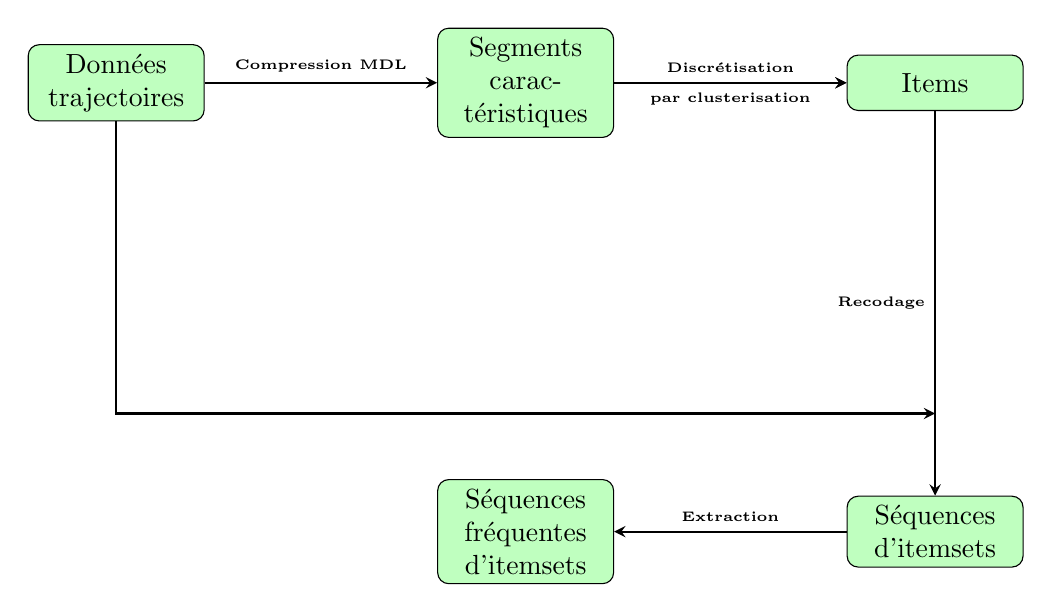
\begin{tikzpicture}[node distance = 2.2cm]
    \node(traj)[terminator]{Données trajectoires};
    \node(segs)[terminator, right of=traj, xshift=3cm]{Segments carac\-téristiques};
    \node(items)[terminator, right of=segs, xshift=3cm]{Items};
    \node(itemsets)[terminator, below of=items, yshift=-3.5cm]{Séquences d'itemsets};
    \node(itemsetsFreq)[terminator, left of=itemsets, xshift=-3cm]{Séquences fréquentes d'itemsets};
    \coordinate (Qf) at ([yshift=1.5cm]itemsets);
    \draw [arrow] (traj) -- node[anchor=south]{\tiny{\textbf{Compression MDL}}}(segs);
    \draw [arrow] (segs) -- node[anchor=south]{\tiny{\textbf{Discrétisation}}}(items);
    \draw [arrow] (segs) -- node[anchor=north]{\tiny{\textbf{par clusterisation}}}(items);
    \draw [arrow] (items) -- node[anchor=east]{\tiny{\textbf{Recodage}}}(itemsets);
    \draw [arrow] (itemsets) -- node[anchor=south]{\tiny{\textbf{Extraction}}}(itemsetsFreq);
    \draw[thick,->,>=stealth,in=180,out=0] (traj) |- (Qf);
\end{tikzpicture}
\caption{Illustration du pipeline.}
\label{pipeline}
\end{figure}

%\include{Pages/Preprocessing}
%\include{Pages/Extraction}
\setlength{\columnsep}{0.6cm}
% \setlength{\columnseprule}{1pt}
\chapter{Réalisation du pipeline}

%K4 <3

% TRACLUS ? présentation ?

\section{Compression de trajectoire}
\label{compression}

Pour permettre une analyse des données par les algorithmes en un temps raisonnable, la compression est une étape importante du traitement. Cependant, il y a un équilibre à trouver entre concision et précision. Pour y arriver, il a été décidé d'adopter le principe MDL (Minimum Description Length) et plus particulièrement, une méthode permettant de trouver une solution approximative en temps linéaire.

Nous nous basons ici sur le travail de \href{https://hanj.cs.illinois.edu/pdf/sigmod07_jglee.pdf}{Jae-Gil Lee et Kyu-Young Whang}~\cite{lee2007trajectory}. 

Pour réaliser cette compression, il faut introduire la notion de distance à choisir, quelles sont les propriétés désirables pour une compression de trajectoire, la formalisation à l'aide du principe MDL. Avant de terminer sur la solution approximative proposée. Cette méthode de compression rapide est nécessaire pour traiter de grandes quantités de données de trajectoires tout en préservant une précision suffisante pour l'analyse ultérieure.

\subsection{Propriétés désirables pour la compression de trajectoire}

L'objectif est de trouver des points caractéristiques tels qu'ils se trouvent à clés dans la représentation de la trajectoire, notamment lors de changements flagrants de direction. Avec l'idée d'un équilibre entre précision et concision. Comme illustré ci-dessous \ref{fig:mdlcost}.

\begin{figure}[ht]
    \centering
    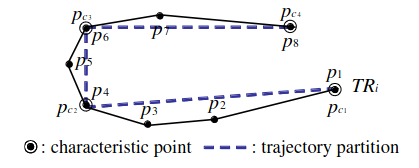
\includegraphics[width=0.5\textwidth]{Images/compressionExample.png}
    \caption{Exemple d'une trajectoire et de sa compression}
    \label{fig:mdlcost}
    Source : \href{https://hanj.cs.illinois.edu/pdf/sigmod07_jglee.pdf}{Trajectory Clustering: A Partition-and-Group Framework}
\end{figure}

\subsection{Fonction de distance}

Pour réaliser du clustering sur des segments de trajectoires, Jae-Gil Lee et Kyu-Young Whang ont défini une notion de distance composée de trois composantes comme suit : la distance perpendiculaire ($d_{\perp}$), la distance parallèle ($d_{\parallel}$) et la distance angulaire ($d_{\theta}$). Elles sont illustrées de manière intuitive dans la Figure~\ref{fig:distances}. Il est possible de voir le détail des calculs en annexe~\ref{an:compression_dist}.

Supposons que nous ayons 2 segments en $n$ dimensions, $L_i = s_i e_i$ et $L_j = s_j e_j$, où $s_i$, $e_i$, $s_j$ et $e_j$ représentent des points de $n$ dimensions. Nous assignons le segment plus long à $L_i$ et le segment plus court à $L_j$.


\begin{figure}[ht]
    \centering
    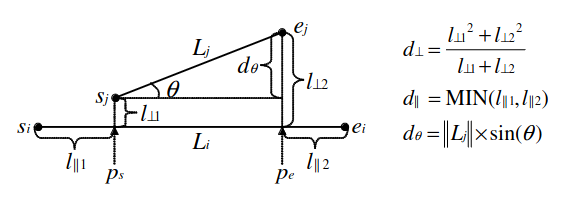
\includegraphics[width=0.44\textwidth]{Images/distances.png}
    \caption{Les 3 composantes de distance entre 2 segments}
    \label{fig:distances}
    Source : \href{https://hanj.cs.illinois.edu/pdf/sigmod07_jglee.pdf}{Trajectory Clustering: A Partition-and-Group Framework}
\end{figure}


\subsection{Principe MDL formalisé}

Le concept de Longueur de Description Minimum (MDL) est largement utilisé en théorie de l'information pour décrire un ensemble de théories et d'applications. L'idée clé de ce concept est que pour un ensemble de données (D) donné, la meilleure hypothèse (H) est celle qui conduit à la meilleure compression pour ces données. Les deux composantes de base de MDL sont : $L(H)$ et $L(D|H)$, où $L(H)$ est la longueur, en bits, de la description de l'hypothèse et $L(D|H)$ est la longueur, en bits, de la description des données lorsqu'elles sont encodées à l'aide de l'hypothèse. La meilleure hypothèse $H$ pour expliquer D est celle qui minimise la somme de $L(H)$ et $L(D|H)$. Ici, $L(H)$ mesure le degré de concision et $L(D|H)$ celui de l'exactitude.

\vspace{0.5cm}

En formalisant ce concept ici :
 \begin{equation}
    L(H) = \sum_{j=1}^{p-1} \log_2(\text{len}(pc_j pc_{j+1}))
\end{equation}

 \begin{equation}
    L(D|H) = \sum_{j=1}^{p-1} \sum_{k=c_j}^{c_{j+1}-1} {\log_2(d_\perp(pc_j pc_{j+1}, pk pk_{k+1})) + \log_2(d_\theta(pc_j pc_{j+1}, pk pk_{k+1}))}
\end{equation}

\begin{figure}[ht]
    \centering
    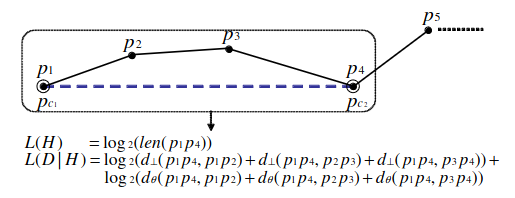
\includegraphics[width=0.6\textwidth]{Images/MDLcostExample.png}
    \caption{Exemple de la formalisation MDL sur un bout de trajecoires}
    \label{fig:mdlcost2}
    Source : \href{https://hanj.cs.illinois.edu/pdf/sigmod07_jglee.pdf}{Trajectory Clustering: A Partition-and-Group Framework}
\end{figure}


\subsection{Méthode de compression rapide en temps linéaire}

La méthode proposée consiste à considérer que l'ensemble des optima locaux est l'optimum global. Cela s'apparente à une observation de l'évolution de l'entropie locale, ici l'équilibre local entre le $L(H)$ et $L(D|H)$, en sélectionnant à chaque étape le point suivant comme point caractéristique. Si l'entropie augmente brusquement, il faut alors sélectionner le point précédent comme point caractéristique et reprendre à partir de celui-ci. Cela s'illustre bien sûr la figure \ref{fig:mdlcost}. Voir annexe pour plus de détails \ref{an:compression_lin}.



\section{Clustering}
\label{clustering}


Le clustering~\ref{fig_clustering} est une technique d'analyse de données qui permet de regrouper des données similaires ensemble en des groupes appelés "clusters". Le but du clustering est d'identifier des structures dans les données qui ne sont pas évidentes à observer à première vue.

Le clustering est une technique non supervisée, ce qui signifie qu'il n'y a pas de variable de réponse prédéfinie. Au lieu de cela, les algorithmes de clustering examinent les caractéristiques des données et les regroupent en fonction de leur similarité. Les données qui sont similaires sont regroupées dans le même cluster, tandis que les données qui sont différentes sont regroupées dans des clusters différents.

Il existe plusieurs types d'algorithmes de clustering, chacun avec ses propres avantages et inconvénients.
Le choix de l'algorithme de clustering dépendra des données et de l'objectif de l'analyse. Les clusters peuvent être utilisés pour découvrir des tendances ou des relations cachées dans les données, ou pour segmenter les clients en fonction de leurs caractéristiques communes.

\begin{figure}[!ht]
    \centering
    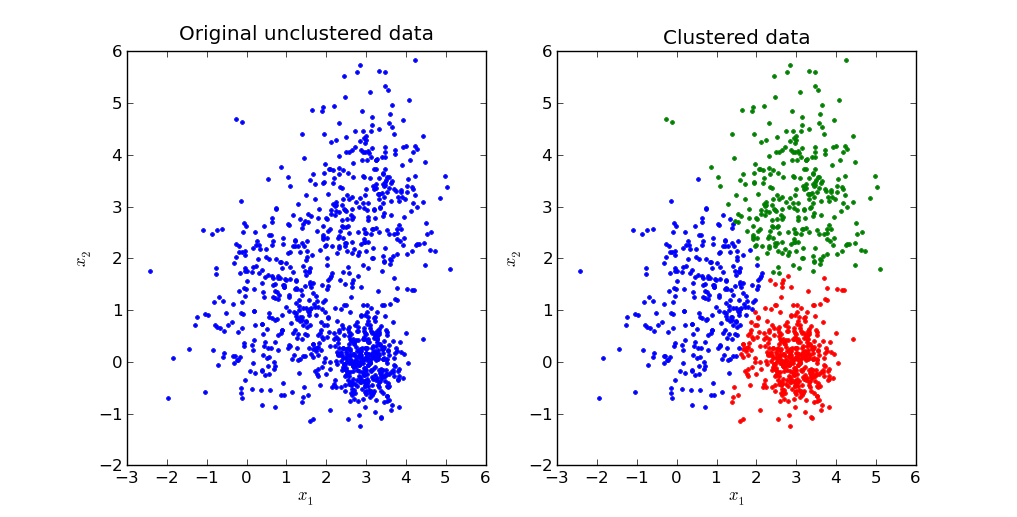
\includegraphics[width=1\textwidth]{Images/clustering.png}
    \caption{Exemple de clustering}
    \label{fig_clustering}
    Source : \href{https://mubaris.com/posts/kmeans-clustering/}{mubaris clustering}
\end{figure}

\newpage

\subsection{K-Means et K-Medoids}
\label{algo_k}
Fonctionnement de K-Means:

\begin{enumerate}
    \item spécifier le nombre de clusters(K).
    \item Ensuite, sélectionner K éléments de données initiaux qui serviront de centres de cluster. Ces éléments peuvent être choisis au hasard ou selon un critère spécifique.
    \item À présent, l'algorithme attribue chaque élément de données au cluster le plus proche en termes de distance. Cela signifie que chaque élément est assigné au centre de cluster le plus proche.
    \item Une fois que tous les éléments de données ont été attribués à un cluster, les centres de cluster sont recalculés en calculant la moyenne de tous les éléments qui leur ont été assignés.
    \item Les étapes 3 et 4 sont répétées jusqu'à ce que les centres de cluster ne changent plus, ou que le nombre d'itérations maximum soit atteint.
\end{enumerate}

À la fin du processus, chaque élément de données appartient à un cluster spécifique, et chaque cluster est caractérisé par son centre. L'algorithme K-means vise à minimiser la somme des distances entre chaque élément de données et son centre de cluster correspondant. C'est ce qu'on appelle la fonction objective de l'algorithme.

L'algorithme K-means est rapide et efficace pour de petits et moyens ensembles de données. Toutefois, il peut être sensible aux éléments de données initiaux sélectionnés au hasard, et il peut avoir du mal à trouver la solution optimale pour de grands ensembles de données ou pour des données ayant une structure complexe.

L'algorithme k-medoids est sensiblement similaire à celui de k-means. La différence étant qu'au lieu de prendre la moyenne du cluster comme centre, il faut prendre l'élément dont la somme des distances par rapport à tous les autres éléments du cluster est la plus petite. Cela permet de rester plus proche des données réelles. Mais cela représente un coût supplémentaire.

\subsection{Propagation d'affinité}
\label{propa}

La propagation d'affinité est un algorithme de clustering proposé par Brendan J. Frey et Delbert Dueck, basé sur des données qui utilise une approche de propagation de similarité entre les points de données pour former des clusters. L'algorithme de propagation d'affinité utilise donc des mesures de similarité entre les points de données pour déterminer les clusters. L'implémentation est décrite en détail dans l'annexe \ref{an:propa}.

\begin{enumerate}

    \item \underline{Initialisation}: initialiser quatre matrices, une pour la similarité, une pour les responsabilités, une pour les disponibilités et une matrice finale qui va nous permettre d'extraire les différents clusters. Ces matrices sont de taille N*N avec N, la taille de l'ensemble d'éléments.
    
    \item \underline{Calcul de la similarité}: calculer la similarité entre chaque paire d'élément de données en utilisant une mesure de similarité, pour ensuite remplir la matrice de similarité. Dans notre cas, nos éléments sont dotés d'une méthode afin de quantifier la distance d'un élément à un autre. L'intérêt de cette matrice est de quantifier à quel degré un élément est semblable à un autre.
    
    \item \underline{Calcul des responsabilités}: l'algorithme utilise ensuite les valeurs de la similarité pour calculer les responsabilités de chaque élément en tenant compte des valeurs de leur disponibilité. Les responsabilités mesurent l'importance d'un élément pour les autres points de données.\\ 
    \begin{figure}[ht]
        \centering
        \begin{equation}
            \begin{aligned}
                R\left ( i,k \right )\leftarrow S\left ( i,k \right ) - max\left \{ D\left ( i,k' \right ) + S\left ( i,k' \right ) \right \}\\
                k'\neq k\\
            \end{aligned}
        \end{equation}
        \caption{Formule de la responsabilité}
        \label{fig:responsibility}
    \end{figure}

    \item \underline{Calcul des disponibilités}: l'algorithme va ensuite utiliser la matrice des responsabilités pour mettre à jour la matrice des disponibilités. Les disponibilités mesurent l'importance des autres points de données pour un élément donné.
    \begin{figure}[ht]
        \centering
        \begin{equation}
            \begin{aligned}
                D\left ( i,k \right )\leftarrow min\left \{ O,R\left ( k,k \right ) + \sum max\left \{ 0,R\left ( i',k \right ) \right \} \right \}\\
                i' \neq i, i' \neq j\\
            \end{aligned}
        \end{equation}
        \caption{Formule de la disponibilité}
        \label{fig:avariability}
    \end{figure}

    \item \underline{Assignation des clusters}: les étapes 3 et 4 vont être réitérées un nombre n de fois dans notre implémentation. Notre algorithme va ensuite venir mettre à jour la matrice finale, souvent appelée matrice de "critère" ou de "préférence", elle assigne chaque élément à un cluster en fonction de la responsabilité maximale de chaque élément. Cette matrice se calcule en faisant le somme matricielle de de responsabilité et de la disponibilité.
    
\end{enumerate}

% \subsubsection{Comment avons-nous implémenté cet algorithme ?}
% Par soucis de lisibilité, notons :


% \begin{itemize}
%     \item S, la matrice de similarité.
%     \item R, la matrice de responsabilité.
%     \item D, la matrice de disponibilité.
% \end{itemize}
% % \begin{multicols}{2}
%     \hspace*{13px} La structure de nos matrices est faite pour pouvoir comparer un élément d'index I à un élément d'index J, il est donc nécessaire d'utiliser une structure de liste ordonnée et fixe.\\
%     Pour commencer, il nous faut remplir la matrice de similarité.
%     Chacun de nos objets donnés est capable au préalable de se comparer à d'autres objets du même type.\\
%     Une méthode distance nous permet donc de comparer un objet I à un objet J. \\ 
%     (Voir l'algorithme implémenté \ref{sec:simcalc})\\
%     % \begin{algorithmic}[1]
%     %     % \State $\texttt{Méthode de calcul de la similarité$
%     %     \State $E \gets \texttt{L'ensemble d'éléments}$
%     %     \State $T \gets \texttt{la taille de E}$
%     %     \State $S \gets \texttt{Une matrice de taille T*T}$
%     %     \For{\texttt{I allant de 0 à T}}
%     %         \For{\texttt{J allant de 0 à T}}
%     %             \State $S(I,J) \gets \texttt{E(I).distance(E(J))}$
%     %         \EndFor
%     %     \EndFor
%     % \end{algorithmic}
% % \end{multicols}

% % \begin{multicols}{2}
%     Mettre à jour la matrice de responsabilité se fait une fois la similarité calculée. (voir figure \ref{fig:responsibility})\\
%     De manière plus explicite, la responsabilité d'un élément i par rapport à k se calcule par sa valeur de similarité, moins la valeur maximale de la disponibilité pour les éléments i en considérant tous les autres points de données j, sauf l'élément k. De cette manière, nous pouvons quantifier l'importance d'un élément pour les autres éléments.\\
%     (Voir l'algorithme implémenté \ref{sec:rescalc})\\
%     % \begin{algorithmic}[1]
%     %     % \State $\texttt{Méthode de calcul de la responsabilité$
%     %     \State $E \gets \texttt{L'ensemble d'éléments}$
%     %     \State $T \gets \texttt{la taille de E}$
%     %     \State $S \gets \texttt{Une matrice de taille T*T}$
%     %     \For{\texttt{I allant de 0 à T}}
%     %         \For{\texttt{J allant de 0 à T}}
%     %             \State $V = \texttt{S[i] + D[i]}$
%     %             \State $V[i] = -\infty$ 
%     %             \State $V[k] = -\infty$
%     %             \State $R[i,k] = R[i,k] + (S[i,k] - max(v))$
%     %         \EndFor
%     %     \EndFor
%     % \end{algorithmic}
    
%     \hspace*{13px} Un paramètre que nous avons nommé "damping" est un paramètre d'amortissement compris entre 0 et 1 qui contrôle la quantité de propagation d'affinité entre les éléments. Nous l'appliquons à la formule de cette manière :\\ 
%     \begin{equation}
%         \begin{aligned}
%             R\left ( i,k \right ) = R\left ( i,k \right ) * damping + S\left ( i,k \right ) - (1 - damping) * max\left \{ D\left ( i,k' \right ) + S\left ( i,k' \right ) \right \}
%         \end{aligned}
%     \end{equation}\\
%     Plus ce paramètre tend vers 0, plus les éléments similaires ne seront regroupés qu'avec leurs voisins directs. Au contraire, plus le damping est proche de 1, plus les points de données similaires seront regroupés ensemble, indépendamment de leur position dans l'ensemble des éléments.\\
    
%     Mettre à jour la matrice de disponibilité se fait une fois la responsabilité mise à jour. \\ 
%     (Voir l'algorithme implémenté \ref{sec:avacalc})\\
%     % \begin{algorithmic}[1]
%     %     \State $E \gets \texttt{L'ensemble d'éléments}$
%     %     \State $T \gets \texttt{la taille de E}$
%     %     \State $R \gets \texttt{Une matrice de taille T*T}$
%     %     \For{\texttt{I allant de 0 à T}}
%     %         \For{\texttt{J allant de 0 à T}}
%     %             \State $V \gets \texttt{prendre colone k dans R}$
%     %             \If{$i\neq k$} 
%     %                 \State $V[i] = -\infty$ 
%     %                 \State $V[k] = -\infty$
%     %                 \State $V[V < 0] = 0$
%     %                 \State $D[i,k] = D[i,k] + min(0, R[k,k] + somme(V))$
%     %             \Else
%     %                 \State $V[k] = -\infty$
%     %                 \State $V[V < 0] = 0$
%     %                 \State $D[k,k] = D[k,k] + somme(V)$
%     %             \EndIf
%     %         \EndFor
%     %     \EndFor
%     % \end{algorithmic}
%     R(k,k) est l'élément de la matrice de responsabilité R correspondant à la similarité entre le point k et lui-même. La somme est prise sur tous les points de données i' autres que i et j, et mesure l'influence des autres points de données sur la disponibilité du point i pour être affecté au 
%     cluster contenant le point j. La fonction max est utilisée ici pour ne prendre en compte que les valeurs positives de la matrice de responsabilité, ne considérant donc que les éléments i' qui ont une similarité positive avec le point k. Enfin, la fonction min est là pour contraindre le résultat final à être négatif ou nul. Cela permet de quantifier l'importance des autres éléments pour un élément donné.\\
%     \hspace*{13px} Une fois le processus de mise à jour de la responsabilité et la disponibilité répété un certain nombre de fois, nous finissons par faire l'addition matricielle de la matrice de responsabilité avec celle de disponibilité pour pouvoir en extraire les clusters et leur représentant, nous appelons cette matrice la matrice de critère. La valeur de critère la plus élevée de chaque colonne est désignée comme exemplaire et les colonnes qui partagent le même exemplaire se trouvent dans le même cluster.\\
%     \hspace*{13px} Le processus de mise à jour de la responsabilité et la disponibilité sont exécutés un nombre arbitrairement de fois dans notre implémentation. Cependant, cet algorithme converge relativement rapidement, calculer la matrice de critère à chaque itération permettrait de détecter une convergence et ainsi éviter de réaliser des itérations inutiles. \\

% \end{multicols}

% \begin{multicols}
    \subsubsection{Quels sont les inconvénients d'un tel algorithme ?}
    \hspace*{13px} L'inconvénient principal de cet algorithme est sa complexité quadratique O(n²). L'algorithme de propagation d'affinité nécessite une grande quantité de mémoire pour stocker ses matrices, qui sont des matrices carrées de la taille de l'ensemble au carré. Pour de grands ensembles de données, cela peut nécessiter une quantité considérable de mémoire, ce qui peut rendre l'exécution de l'algorithme difficile, voire impossible sur des ordinateurs avec une mémoire limitée.\\
    Le temps d'exécution est lui aussi impacté par la taille du jeu de donnée à traiter.
    
    \subsubsection{Quels en sont les avantages ?}
    
    \hspace*{13px} Bien que la complexité de cet algorithme puisse réduire le nombre d'applications de cet algorithme, son principal avantage est que contrairement aux méthodes de clustering traditionnelles, propagation d'affinité n'a pas besoin de connaitre le nombre de clusters à assigner, il va automatiquement le trouver tout en gardant une certaine pertinence des résultats.\\
    Malgré sa complexité, les calculs des matrices de cet algorithme sont parallélisables, rendant le calcul de celles-ci moins contraignantes sur de grands jeux de données.\\
    Une autre optimisation de cet algorithme est d'implémenter les itérations en calcul matriciel au lieu d'utiliser des boucles, rendant le calcul bien moins couteux en temps.
    
sources :\\
\href{https://utstat.toronto.edu/reid/sta414/frey-affinity.pdf}{Rapport de Brendan J. Frey et Delbert Dueck}\\
\href{https://github.com/scikit-learn/scikit-learn/blob/main/sklearn/cluster/_affinity_propagation.py}{Implémentation faite par la librairie  scikit-learn}\\
\href{https://towardsdatascience.com/unsupervised-machine-learning-affinity-propagation-algorithm-explained-d1fef85f22c8}{Publication de Towards Data Science}\\

%%%%%%%%%%%%%%%%%%%%%%%%%%%%%%%%%%%%%%%%%%%%%%%%%%%%
%\newpage

\section{Extraction de connaissance dans les données}
\label{extraction}

L'extraction de connaissance est le processus d'extraction d'informations utiles et exploitables à partir de sources de données brutes et non structurées, telles que des documents, des bases de données, des fichiers texte, des images, des vidéos et d'autres types de médias numériques.\\
Les principales taches de l'extraction des données sont le \textbf{clustering}, l'analyse des valeurs \textbf{aberrantes}, la \textbf{classification} et l'\textbf{extraction de motif fréquents}.
\subsection{Extraction séquentielle}
L'extraction séquentielle est une technique d'analyse de données qui consiste à identifier des motifs séquentiels récurrents dans une série temporelle ou une séquence d'événements.\\
Plus précisément, l'extraction séquentielle recherche des sous-séquences qui se produisent fréquemment dans une séquence donnée et les identifie comme des motifs significatifs. Ces motifs peuvent ensuite être utilisés pour comprendre le comportement de la séquence, pour prédire des événements futurs, pour détecter des anomalies ou pour d'autres applications.\\
Par exemple, si l'on analyse les achats d'un client sur une période, l'extraction séquentielle pourrait identifier des motifs tels que "le client achète toujours du café après avoir acheté du lait". Cela pourrait aider une entreprise à mieux comprendre les préférences du client et à proposer des offres ciblées.\\
En résumé, l'extraction séquentielle est une technique utile pour trouver des modèles récurrents dans une série temporelle ou une séquence d'événements, ce qui peut aider à mieux comprendre le comportement et à prendre des décisions éclairées en conséquence.
\subsubsection{Exemple}
\begin{figure}[ht!]
    \centering
    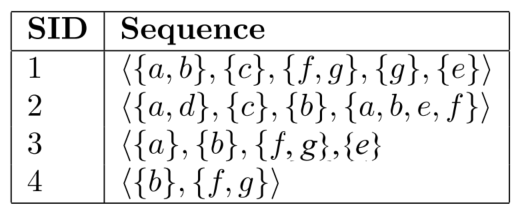
\includegraphics{Images/seq2-1.png}
    \caption{Exemple de séquence d'items}
    \label{fig:seq}
    source : \href{https://data-mining.philippe-fournier-viger.com/wp-content/uploads/2017/03/seq2-1.png}{The data mining blog}
\end{figure}
Dans cet exemple \ref{fig:seq}, les données en question contiennent quatre séquences de transactions d'achats effectuées par différents clients. Chaque séquence représente les articles achetés par un client à différents moments. Une séquence est une liste ordonnée d'ensembles d'articles achetés ensemble, appelés itemsets.\\
Dans cet exemple \ref{fig:seq}, la première séquence (identifiée par SID 1) indique que le client a acheté des articles a et b ensemble, puis a acheté l'article c seul, ensuite a acheté les articles f et g ensemble, puis a acheté l'article g seul, et enfin a acheté l'article e seul.\\
Dans cet exemple \ref{fig:seq}, nous pouvons noter que le pattern séquentiel $\langle$\{a\},\{f,g\}$\rangle$ qui apparait dans deux transactions une et deux, elle est donc un motif fréquent avec un support de 2, le support étant le nombre de transactions contenant cette séquence. De même, nous pouvons voir le pattern $\langle$\{a\},\{g\}$\rangle$ est un motif fréquent avec un support de 3, car apparaissant dans les transactions 1, 2 et 3.\\

Dans notre situation, nous cherchons donc des motifs fréquents qui illustreront les déplacements des joueurs lors des games. Par exemple, si le pattern $\langle$\{A\},\{F\},\{R\}$\rangle$ exprimant les positions du joueur est motif qui apparait de manière fréquente lors des games, il exprimera le fait que si le joueur se trouve (appartient) à un moment T au cluster A il ira ensuite au cluster F, puis B avec un certain  niveau de confiance, avec la confiance représentant la probabilité de réalisation.

\chapter{Expérimentations et Discussion}
\section{Compression}


Les résultats obtenus lors de la compression illustrent l'efficacité de la méthode proposée pour identifier les points caractéristiques d'une trajectoire. En effet, cette méthode nous permet d'atteindre une réduction moyenne de 67.9\% de toutes nos trajectoires. Ces résultats soulignent l'importance de notre approche pour la compression de trajectoires, tout en maintenant leur qualité, comme illustré ici~\ref{fig:traj_versus}.

\begin{figure}[h!]
    \centering
    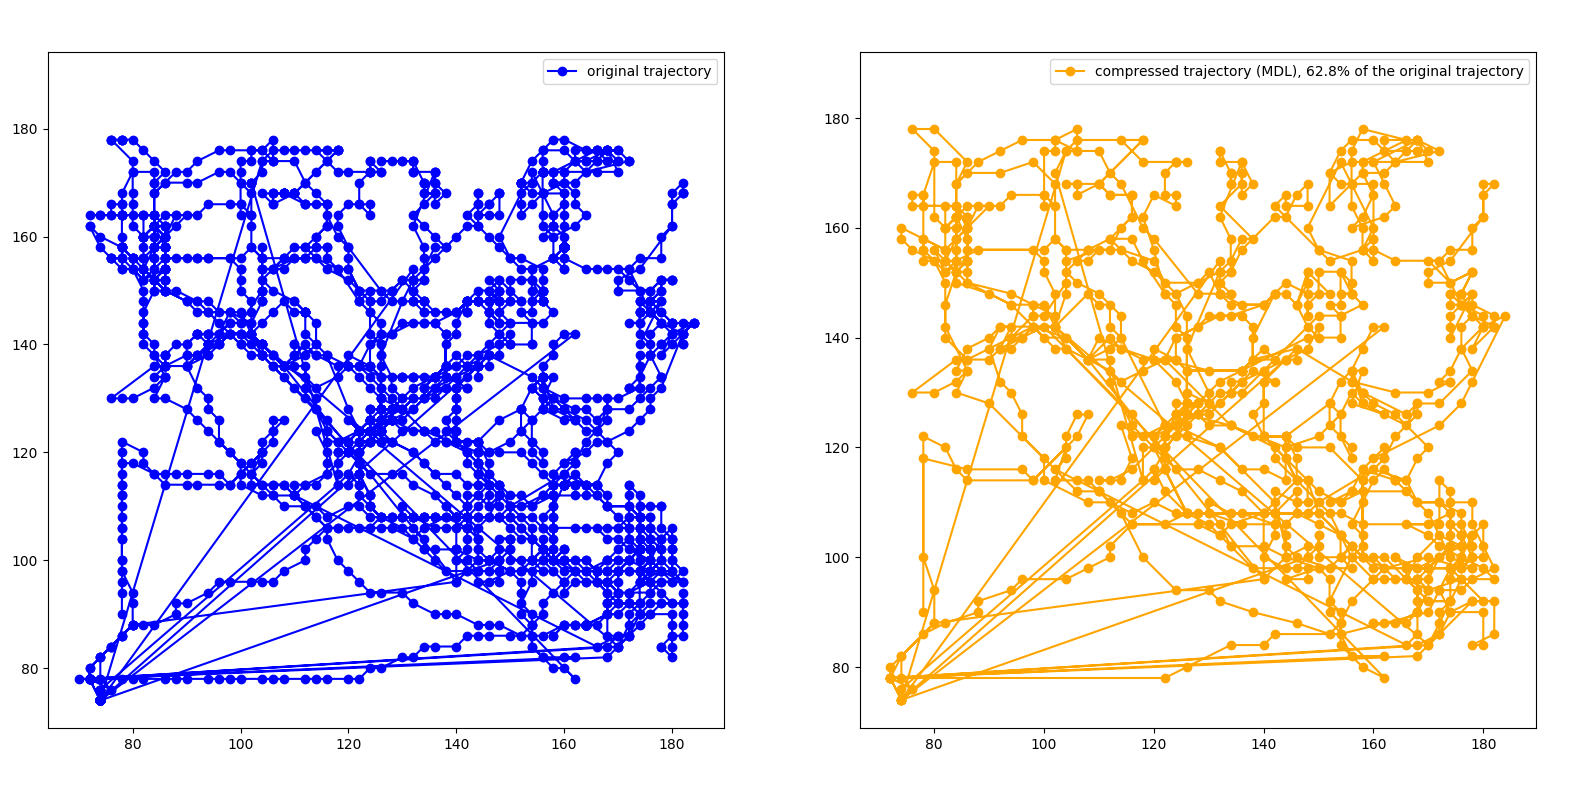
\includegraphics[width=0.8\textwidth]{Images/compVSorigAll.png}
    \caption{Exemple d'une trajectoire avant et après compression}
    \label{fig:traj_versus}
\end{figure}

Il est possible d'observer plus finement l'équilibre entre concision et précision que permet cette méthode sur la figure suivante~\ref{fig:traj_versus100}.

\begin{figure}[h!]
    \centering
    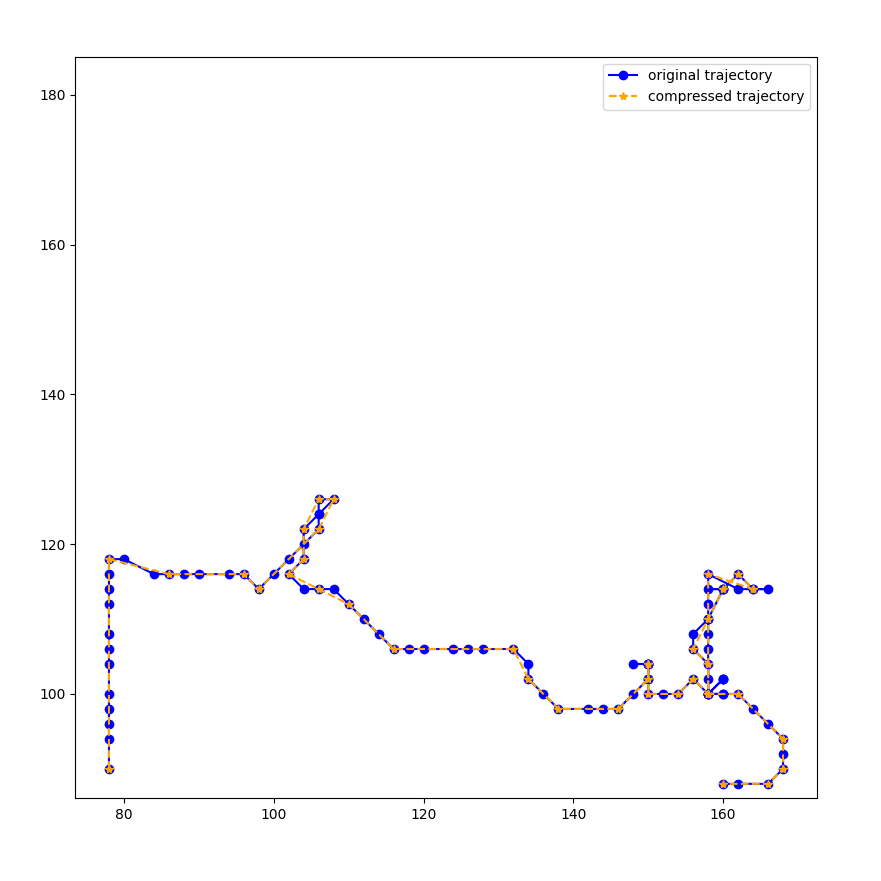
\includegraphics[width=0.5\textwidth]{Images/compVSoriginal100.png}
    \caption{Exemple de la compression sur les 100 premiers points d'une trajectoire}
    \label{fig:traj_versus100}
\end{figure}
\newpage
\section{Clustering}

%Le clustering est une technique d'apprentissage automatique qui consiste à regrouper des données similaires en fonction de leur proximité les unes des autres. 
Pour réaliser un clustering de qualité, il faut d'abord se pencher sur l'étude des paramètres existants. Dans notre cas, il s'agira de l'évaluation de la distance entre deux segments orientés et du nombre de clusters.

Afin d'illustrer plus parlant, il a été décider de se concentrer uniquement sur les trajectoires de l'équipe de gauche.

\textbf{Note}~: Les résultats obtenus avec la méthode de propagation d'affinité présentent un biais significatif en raison de sa complexité spatiale et temporelle, qui suit une complexité en $O(n^2)$. Ainsi, même après compression, le volume important de segments rend difficile son exécution pour plus de deux parties.

\subsection{Paramétrisation de la distance entre segments}

La distance utilisée est la somme pondérée de trois distances~: distance angulaire, distance perpendiculaire et distance parallèle. Les coefficients de cette somme ayant un impact significatif sur les résultats de cette partie, il est nécessaire d'évaluer, de trouver le paramétrage le plus pertinent. 

Pour cette partie, il a été choisi de fixer le nombre de clusters à 100 pour k-means et k-medoids. Il a été remarqué que cela n'avait pas d'impact particulier sur le paramétrage de la distance.

Pour y arriver, plusieurs expérimentations ont été menées successivement afin d'observer les variations qu'impliquent les paramètres pour chaque algorithme. Une fois ce tour d'horizon réalisé, il est possible d'orienter les choix plus précisément. 

\subsubsection{k-means}



\begin{figure}[h!]
    \centering
    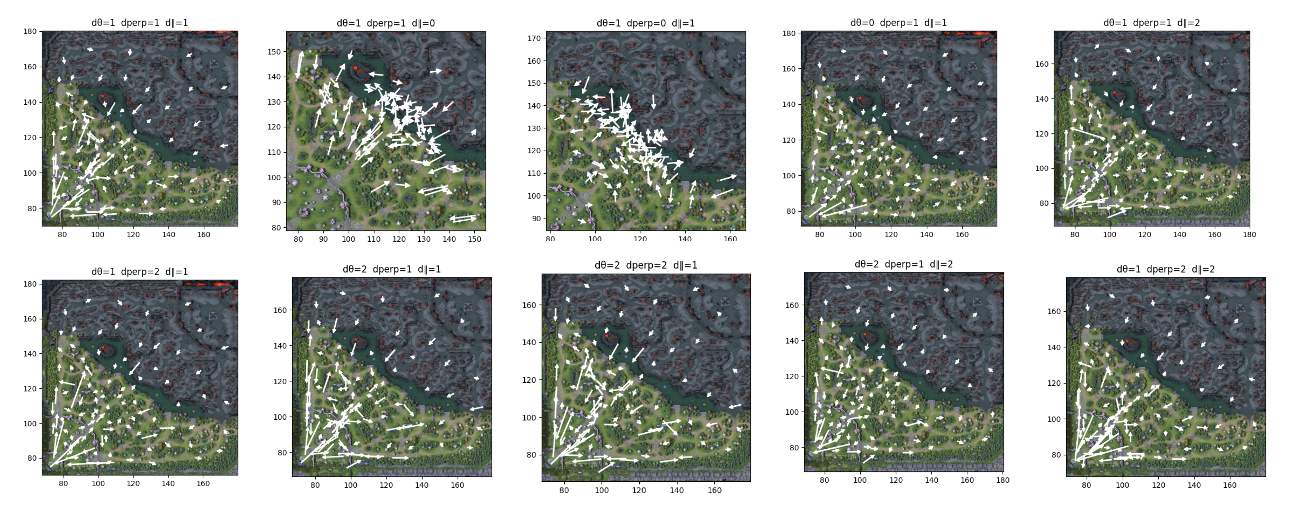
\includegraphics[width=0.9\textwidth]{Images/kmeans/kmeans_seq.png}
    \caption{Résultats clustering k-means pour différentes paramétrisations de la distance}
    \label{fig:kmeans_seq}
\end{figure}

Sur ces résultats \ref{fig:kmeans_seq}, il est possible de distinguer nettement les différences existantes entre chacune des paramétrisations. Lorsque son facteur est égal à 0, a distance angulaire est critique pour obtenir des résultats couvrant correctement les trajectoires sur toute la carte. C'est également le cas pour la distance perpendiculaire. Concernant la distance parallèle, il semblerait qu'elle permette d'affiner le groupement de segments de même orientation et obtenir des segments représentatifs plus longs sur les morceaux de trajectoire récurrents. Cet équilibrage est ici le plus pertinent avec l'adoption d'un facteur 1/2 pour la distance parallèle.

En partant de ces observations, il est apparu qu'un facteur de 1/5 pour la distance parallèle et de 1 pour les deux autres distances donnait des résultats satisfaisant  Comme illustré ici \ref{fig:kmeans_5_5_1}.

\begin{figure}[h!]
    \centering
    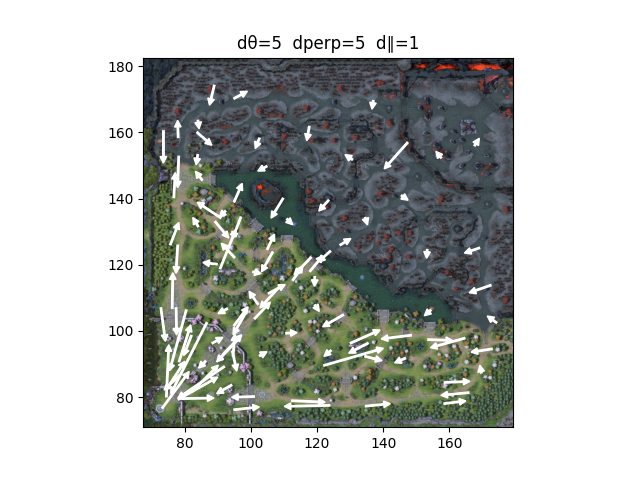
\includegraphics[width=0.6\textwidth]{Images/kmeans/kmeansdBis_5_5_1.png}
    \caption{Résultat clustering k-means avec un facteur parallèle de 1/5}
    \label{fig:kmeans_5_5_1}
\end{figure}


\newpage
\subsubsection{k-medoid}
\begin{figure}[h!]
    \centering
    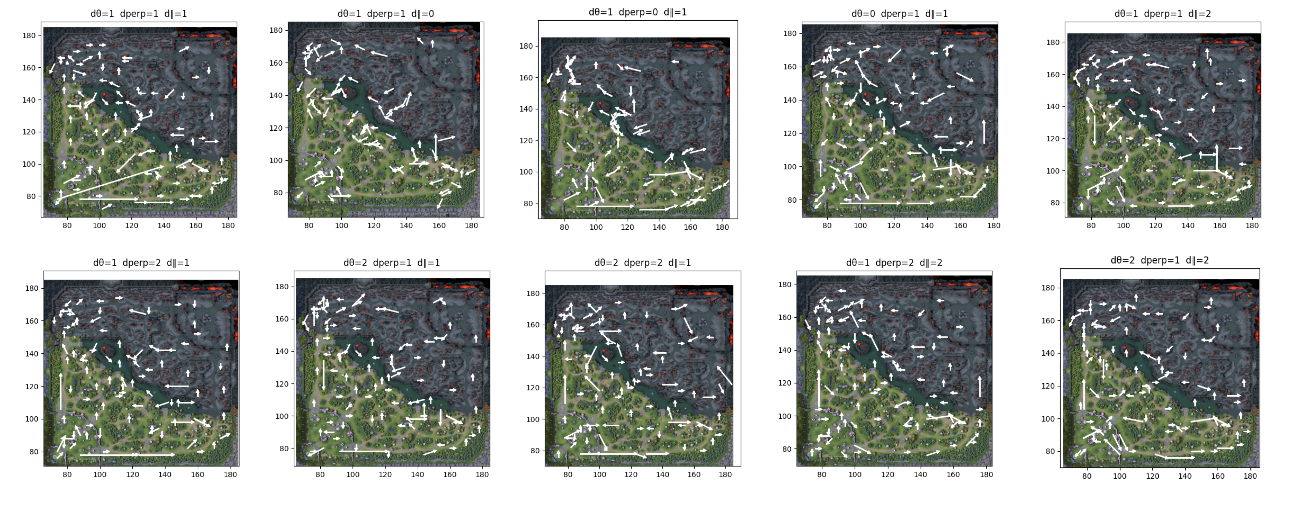
\includegraphics[width=0.9\textwidth]{Images/kmedoid/kmedoid_variationsV2.png}
    \caption{Résultats clustering k-medoids pour différentes paramétrisations de la distance}
    \label{fig:kmed_seq}
\end{figure}

Les résultats des tests \ref{fig:kmed_seq} ont montré que le clustering effectué par k-medoid reste relativement constant. Les trois distances jouent un rôle crucial et aucune des trois ne vraiment être négligée. \\
La distance parallèle et perpendiculaire jouent le rôle le plus important en permettant une distribution plus homogène des clusters sur la carte. En effet, elles permettent la prise en compte de trajectoires représentants des mouvements directes sur une durée plus grande\\
La distance angulaire  permet une meilleure différentiation des trajectoires de direction proches.

Au vu de ces résultats, il semble que partir sur un quasi-équilibre entre les trois distances est la meilleure stratégie à adopter afin d'obtenir les meilleurs résultats \ref{fig:kmed_op}.
\begin{figure}[h!]
    \centering
    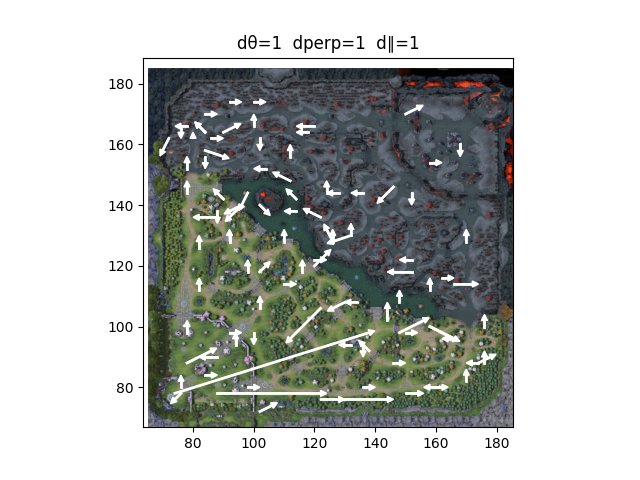
\includegraphics[width=0.6\textwidth]{Images/kmedoid/kmed1_1_1_1.png}
    \caption{K-medoids avec un parametrage de 1 1 1}
    \label{fig:kmed_op}
\end{figure}


\subsubsection{propagation d'affinité}

Pour propagation d'affinité, les résultats \ref{fig:propa_seq} sont globalement assez similaires et traduisent davantage une notion de position que de partitions de trajectoire. En effet, les segments sont généralement courts et répartis sur l'ensemble de la carte de façon homogène. De plus, il y a une tendance à obtenir des segments caractéristique qui sont verticaux, horizontaux ou diagonal.

Néanmoins, il faut prendre en compte que ces résultats sont sujets au biais du faible nombre de parties. De la même façon, cet algorithme possède des paramètres propres, comme le damping, mesure d'acceptance, qui vient affecter le nombre de clusters trouvé.

Ici, il a été choisir d'utiliser un damping de 0.9 avec 60 itérations pour chaque expérimentation.

\begin{figure}[h!]
    \centering
    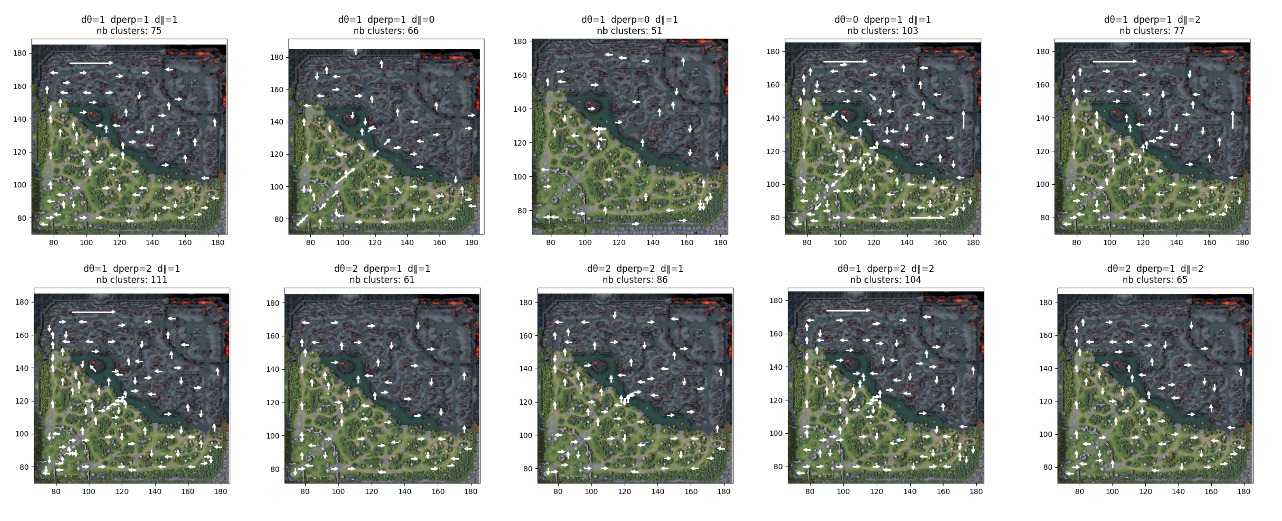
\includegraphics[width=0.9\textwidth]{Images/propa/propa_variations.png}
    \caption{Résultats clustering propagation d'affinités pour différentes paramétrisations de la distance}
    \label{fig:propa_seq}
\end{figure}

Au vu de ces résultats, le plus pertinent reste la mise à 0 du facteur d'angle, comme sur la figure \ref{fig:propa_011}.

\begin{figure}[h!]
    \centering
    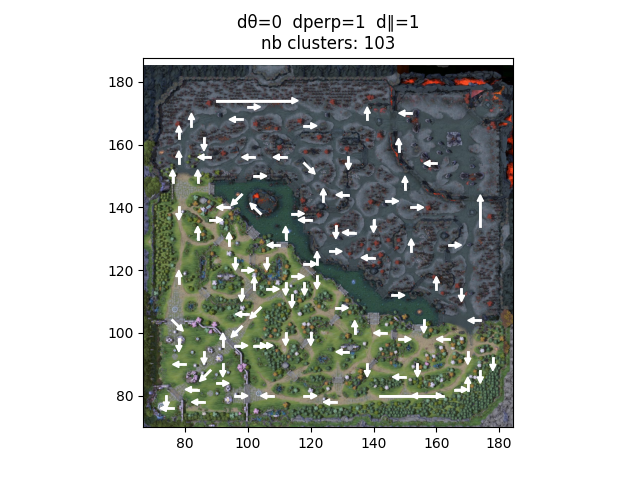
\includegraphics[width=0.6\textwidth]{Images/propa/propa4_0_1_1.png}
    \caption{Résultat clustering propagation d'affinité avec un facteur d'angle de 0}
    \label{fig:propa_011}
\end{figure}



\subsubsection{Discussion}

Il est notable que la paramétrisation a des effets différents sur chacune des méthodes. Cela est assez étonnant dans le cas de k-means et k-medoids, mais la différence s'explique par la différence fondamentale entre les deux algorithmes, ce qui donne aussi sa qualité à k-medoids.

Il est cependant difficile de les comparer avec propagation d'affinités, car celui-ci va également faire une estimation du nombre correct de clusters, en plus de son biais initial lié à son nombre de parties traitées.
% A VERIFIER AVEC LES RESULTATS DEMAIN MATIN

Également, il est intéressant d'observer les différences dans les représentations des trajectoires de chaque côté de la carte, avec des petits segments dans la moitié de carte ennemi (droite), et de longs segments orientés à gauche. Les courts segments semblent représenter des positions sur un espace de la carte \ref{fig:short}. Tandis que les segments orientés allongés semble représenter des trajectoires fréquentes avec une direction précise \ref{fig:long}. 

\begin{figure}[h!]
     \centering
     \begin{subfigure}[b]{0.4\textwidth}
         \centering
         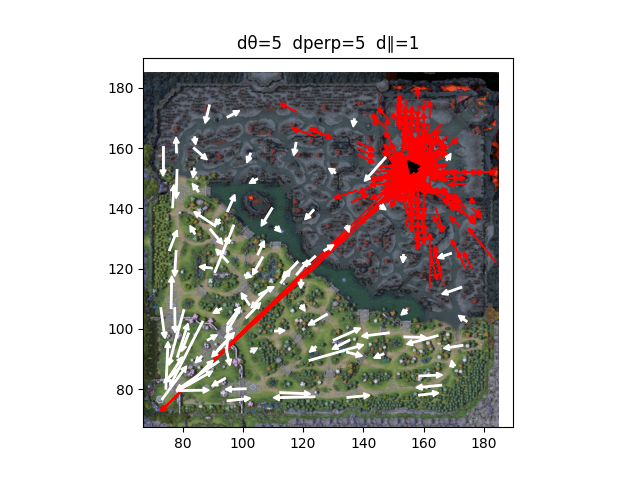
\includegraphics[width=\textwidth]{Images/kmeans/kmeansdBis_show_cluster_short.png}
         \caption{k-means}
         \label{fig:kmean_short}
     \end{subfigure}
     \hfill
     \begin{subfigure}[b]{0.4\textwidth}
         \centering
         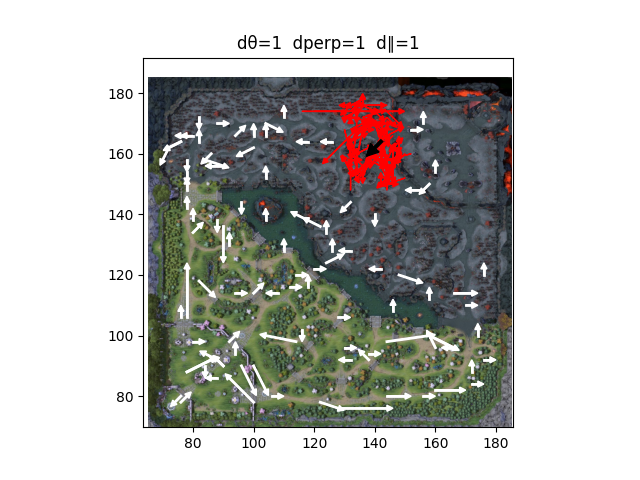
\includegraphics[width=\textwidth]{Images/kmedoid/kmed_212_show_cluster_short.png}
         \caption{k-medoids}
         \label{fig:kmed_short}
     \end{subfigure}
     
     En noir le représentant et en rouge les représentés.
     \caption{Illustration d'un représentant jugé "positionnel"}
     \label{fig:short}
\end{figure}

\begin{figure}[h!]
     \centering
     \begin{subfigure}[b]{0.4\textwidth}
         \centering
         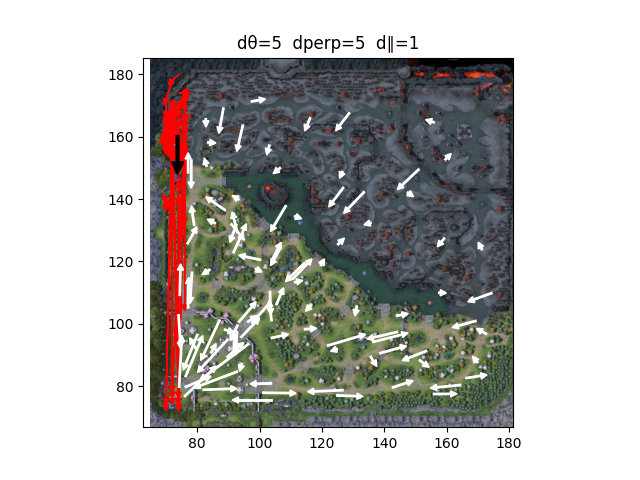
\includegraphics[width=\textwidth]{Images/kmeans/kmeans_long_traj.png}
         \caption{k-means}
         \label{fig:kmean_long}
     \end{subfigure}
     \hfill
     \begin{subfigure}[b]{0.4\textwidth}
         \centering
         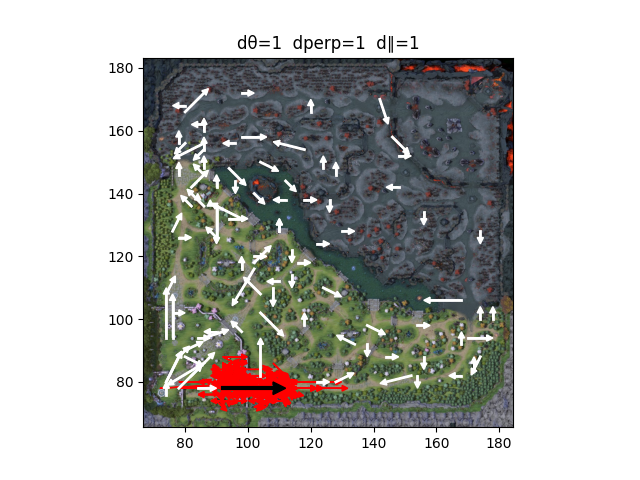
\includegraphics[width=\textwidth]{Images/kmedoid/kmed_long_traj.png}
         \caption{k-medoids}
         \label{fig:kmed_long}
     \end{subfigure}

     En noir le représentant et en rouge les représentés.
     \caption{Illustration d'un représentant de trajectoires}
     \label{fig:long}
\end{figure}
% tmp sans propa

% tmp sans propa

En terme d'information de jeu, il est possible d'interpréter ces différences. Quant aux trajectoires possibles de chaque côté de la carte, cela s'explique pour deux raisons~: premièrement, il est normal pour une équipe de rester de son côté de la carte. Deuxièmement, cela peut s'expliquer par le fait que les excursions du côté adverse de la carte se fait moins souvent et sous la contrainte des déplacements des adversaires, ce qui les rend moins réguliers et moins précis d'une partie à l'autre. 


\subsection{Paramétrisation du nombre de clusters}

Les algorithmes de k-clusters tels que k-means et k-medoids ont un inconvénient notable : ils nécessitent la spécification préalable du nombre de clusters souhaités, ce qui peut entraîner des résultats insatisfaisants en raison de la difficulté à déterminer le nombre optimal de clusters et à choisir une discrétisation adaptée. Bien que l'algorithme de propagation d'affinité soit une alternative intéressante à ce problème, il est difficile de comparer ses résultats avec ceux des autres algorithmes, en raison des différences dans la paramétrisation des distances et du nombre de clusters, comme l'ont montré les résultats précédents.

% L'inconvénient notable des algorithmes de k-clusters, comme k-means et k-medois, est qu'il faut spécifier soit même les nombres de clusters voulus à l'avance. Ce n'est pas optimal, car cela implique souvent de chercher à tâtons, sans garanti de trouver quelque chose de satisfaisant, soit de réaliser une discrétisation trop forte ou trop faible. C'est normalement ici que propagation d'affinité est un algorithme intéressant. Cependant, au vu des résultats précédents sur la paramétrisation des distances qui illustre les différences entre les algorithmes, sans même parler du nombre de clusters, il va être difficile de comparer ces résultats. 

%Une fois avoir déterminé la direction à prendre sur choix des paramètres de la distance, l'étape suivante consiste à déterminer le nombre de clusters permettant d'avoir des résultats de plus grande pertinence.

%\textbf{Note}~: cette partie ne traite pas de la propagation d'affinité, car cet algorithme calcule automatiquement le nombre de clusters à utiliser. Toutefois, il est intéressant de noter que lors de nos expérimentations, nous avons observé une tendance à la diminution puis à la stabilisation du nombre de clusters avec l'augmentation du nombre d'itérations.

Il a été choisi de prendre les meilleurs paramètres de distance pour chaque algorithme pour obtenir une évaluation plus intéressante pour chacun de ces cas.

\subsubsection{k-means}

Au vu des résultats de la figure \ref{fig:kmean_nb}, il est visible qu'à partir de 200 clusters, plusieurs représentants se chevauchent, rendant la discrétion moins intéressante. Cependant, un bon équilibre semble atteint pour un nombre de 150 clusters (figure \ref{fig:kmeans_150}), où il est possible de suivre les trajectoires fréquentes sans que la carte, sans observer trop de chevauchements sur représentants.

\begin{figure}[h!]
     \centering
     \begin{subfigure}[b]{0.35\textwidth}
         \centering
         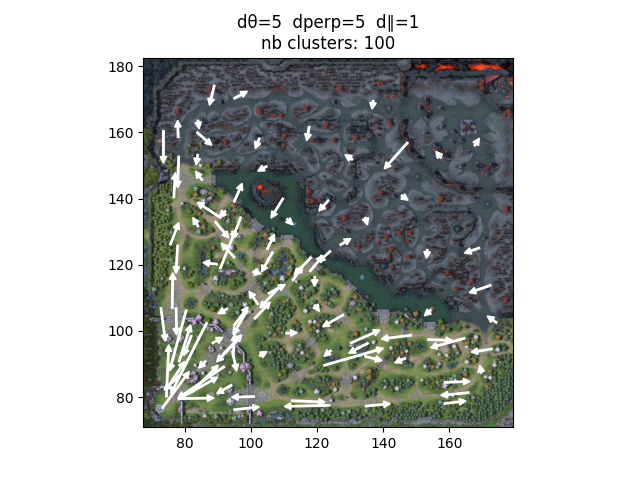
\includegraphics[width=\textwidth]{Images/kmeans/kmeans_100.png}
         \caption{100 clusters}
         \label{fig:kmean_100}
     \end{subfigure}
     %\hfill
     \begin{subfigure}[b]{0.35\textwidth}
         \centering
         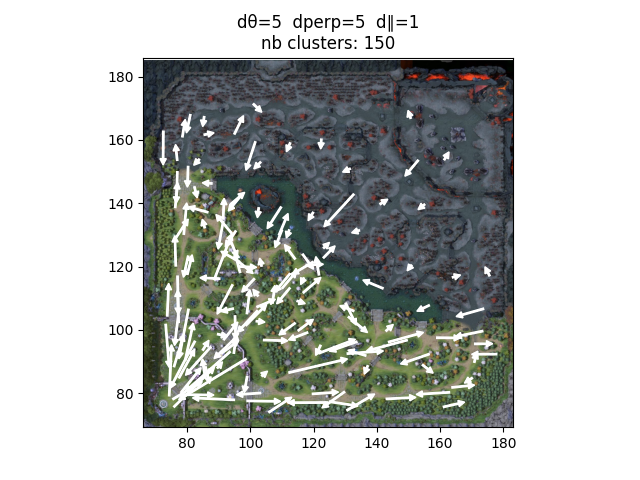
\includegraphics[width=\textwidth]{Images/kmeans/kmeans_150.png}
         \caption{150 clusters}
         \label{fig:kmeans_150}
     \end{subfigure}
     \begin{subfigure}[b]{0.35\textwidth}
         \centering
         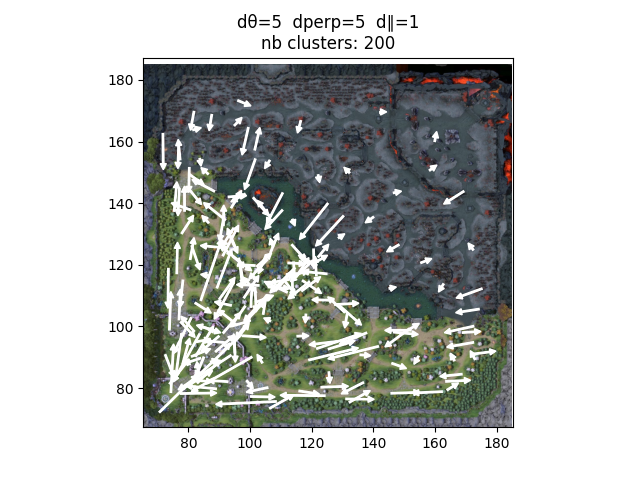
\includegraphics[width=\textwidth]{Images/kmeans/kmeans_200.png}
         \caption{200 clusters}
         \label{fig:kmean_200}
     \end{subfigure}
     %\hfill
     \begin{subfigure}[b]{0.35\textwidth}
         \centering
         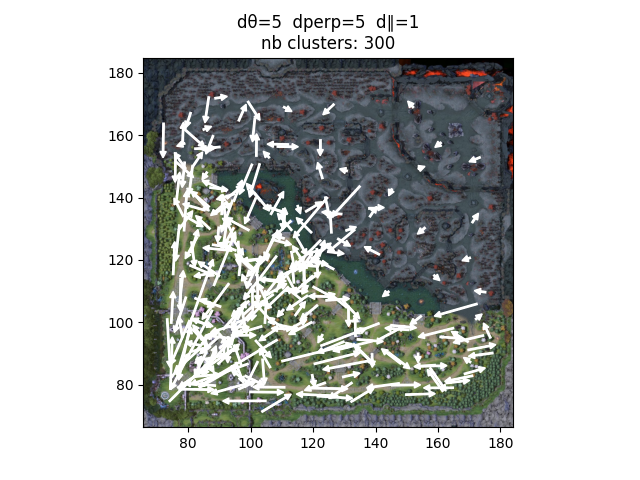
\includegraphics[width=\textwidth]{Images/kmeans/kmeans_300.png}
         \caption{300 clusters}
         \label{fig:kmeans_300}
     \end{subfigure}
     \caption{Évolution de k-means en fonction du nombre de clusters}
     \label{fig:kmean_nb}
\end{figure}


\subsubsection{k-medoids}

Les résultats \ref{fig:kmed_nb} montrent que la qualité de l'information tirée des clusters s'améliore avec leur nombre, mais au-delà de 200 clusters, la quantité d'informations devient trop importante pour en tirer des conclusions. Ainsi, un nombre de 200 clusters semble être un compromis acceptable pour k-medoids afin de suivre l'évolution des trajectoires et détecter les zones à forte fréquentation.
\begin{figure}[h!]
     \centering
     \begin{subfigure}[b]{0.24\textwidth}
         \centering
         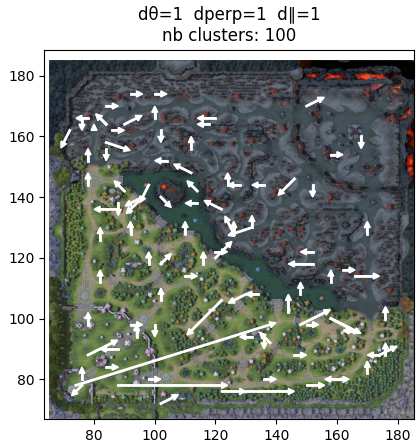
\includegraphics[width=\textwidth]{Images/kmedoid/kmed_100.png}
         \caption{100 clusters}
         \label{fig:kmed_100}
     \end{subfigure}
     \hfill
     \begin{subfigure}[b]{0.24\textwidth}
         \centering
         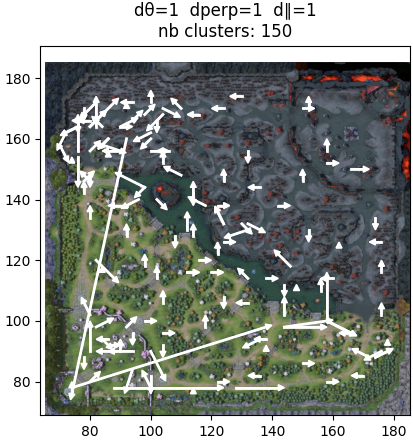
\includegraphics[width=\textwidth]{Images/kmedoid/kmed_150.png}
         \caption{150 clusters}
         \label{fig:kmed_150}
     \end{subfigure}
     \hfill
     \begin{subfigure}[b]{0.24\textwidth}
         \centering
         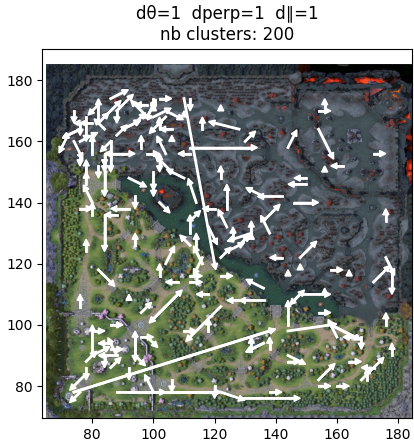
\includegraphics[width=\textwidth]{Images/kmedoid/kmed_200.png}
         \caption{200 clusters}
         \label{fig:kmed_200}
     \end{subfigure}
     \hfill
     \begin{subfigure}[b]{0.24\textwidth}
         \centering
         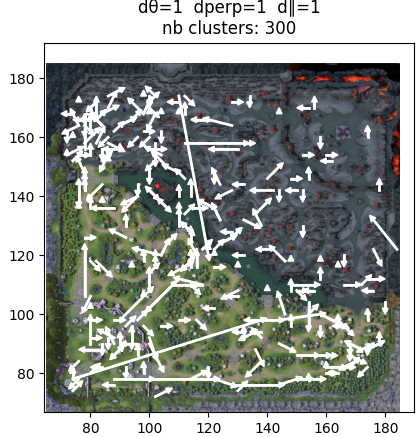
\includegraphics[width=\textwidth]{Images/kmedoid/kmed_300.png}
         \caption{300 clusters}
         \label{fig:kmed_300}
     \end{subfigure}
     \caption{Évolution de k-medoids en fonction du nombre de clusters}
     \label{fig:kmed_nb}
\end{figure}

\subsubsection{propagation d'affinité}

La particularité de propagation d'affinité est justement d'évaluer le nombre de clusters idéal par lui-même. Sur ses meilleurs résultats (figue \ref{fig:propa_011}), nous avons obtenu un nombre de 103 clusters. Cependant, il faut rappeler que ce résultat est aussi lié au facteur de damping et au nombre d'itérations, que nous n'avons pas fait varier. 

\subsubsection{Discussion}

Là encore, les résultats optimaux pour chacun des algorithmes diffèrent. Cela s'explique par leurs différences de paramétrage qui vont influer sur leur définition de représentants. 

Malgré tout, concernant k-means et k-medoids, cela illustre d'autant plus leur différence de fonctionnement, en effet, la capacité de k-medoid à converger qualitativement sur des trajectoires fréquentes font qu'il est possible d'affiner la discrétisation sans brouiller nos résultats. 

L'idéal aurait été d'utiliser la capacité de propagation à trouver le nombre correct de clusters, mais cela s'avère difficile ici. En effet, il aurait fallu que les algorithmes possèdent un paramétrage optimal équivalent. De plus, il aurait fallu à la fois surmonter la contrainte matérielle pour utiliser pleinement propagation d'affinité et mener une étude sur le facteur optimal de damping à utiliser.

\section{Extraction séquentielle}
\subsubsection{Paramètres de l'extraction}
L'algorithme d'extraction séquentiel utilisé \cite{hirate2006generalized} permet l'extraction de motifs fréquents. Plusieurs paramètres rentrent alors en compte.
\begin{enumerate}
    \item \textbf{minsup(minimum support)}~: le nombre minimum de transactions ou doivent apparaître un motif fréquent.
    \item \textbf{min\_time\_interval}~: le temps minimal permis séparant deux itemsets successifs dans un motif.
    \item \textbf{max\_time\_interval}~: le temps maximal permis séparant deux itemsets successifs dans un motif.
    \item \textbf{min\_whole\_interval}~: le temps minimal permis séparant le premier itemset et le dernier itemset d'un motif fréquent (taille minimale du motif).
    \item \textbf{max\_whole\_interval}~: le temps maximal permis séparant le premier itemset et le dernier itemset d'un motif fréquent (taille maximale du motif).
\end{enumerate}

\subsection{Résultats}

Concernant l'extraction, beaucoup de paramétrage ont été testés, mais malgré tout, peu de résultats concluants ont pu être obtenus dans le temps imparti. 

Pour commencer, un découpage arbitraire a été expérimenté. De 30 à 120 secondes, pour finalement rester sur une moyenne de 60 secondes. 

Dès lors, nous avons eu des problèmes d'extraction n'ayant pas spécialement d'intérêt où nous avions des morceaux de trajectoires qui ne se suivaient pas du tout et provenant très probablement de 2 joueurs différents, comme illustré sur la figure \ref{fig:extraction_bad}, il a été décidé de se concentrer sur la trajectoire d'un joueur à la fois.

Ensuite, après les obtentions de résultats illustrant très largement des suites successives de la même trajectoire, nous avons voulu faire varier l'intervalle de temps entre chaque transaction étudié dans l'idée d'éviter le cas où la vitesse ou le rythme des positions des joueurs sur chaque morceau de trajectoire rendrait impossible l'extraction de motifs d'une taille supérieure à 2. Comme illustré sur la figure \ref{fig:interval}. Même si cela pourrait engendrer une perte d'information, il a quand même était jugé nécessaire.

\begin{figure}[h!]
     \centering
     \begin{subfigure}[b]{0.44\textwidth}
         \centering
         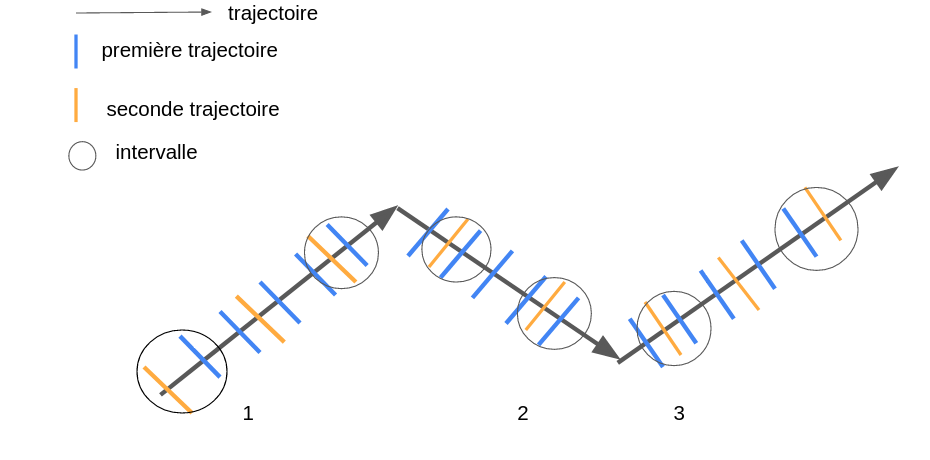
\includegraphics[width=\textwidth]{Images/interval_1.png}         
     \end{subfigure}
     \hfill
     \begin{subfigure}[b]{0.44\textwidth}
         \centering
         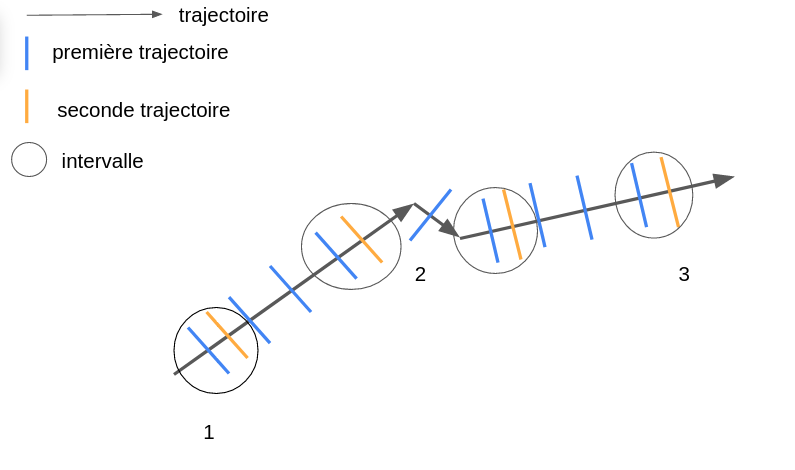
\includegraphics[width=\textwidth]{Images/interval_2.png}
     \end{subfigure}
     \caption{intervalle de temps}
     \label{fig:interval}
\end{figure}     

À ce moment-là, il a été possible d'extraire des motifs formés d'une suite de morceau de trajectoire, exemple figure \ref{fig:extraction_good}, mais ces résultats n'ont pu être obtenus qu'avec un support minimum assez faible (5\%), ce qui n'était pas très satisfaisant. Cependant, il n'était toujours pas possible d'extraire des motifs composés de plus de 2 segments.

\begin{figure}[h!]
     \centering
     \begin{subfigure}[b]{0.44\textwidth}
         \centering
         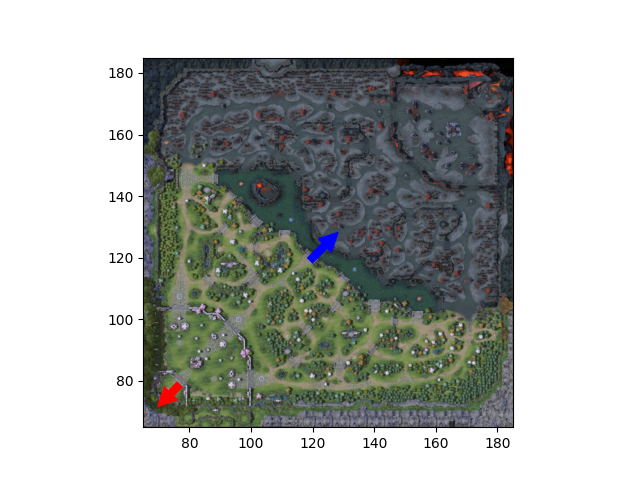
\includegraphics[width=\textwidth]{Images/bad_seq2.png.png}
          \caption{résultat incorrect}
          \label{fig:extraction_bad}
     \end{subfigure}
     \hfill
     \begin{subfigure}[b]{0.44\textwidth}
         \centering
         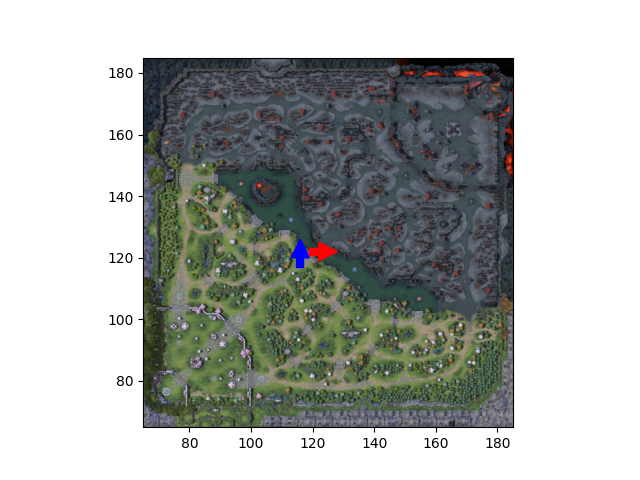
\includegraphics[width=\textwidth]{Images/good_seq2.png.png}
     \caption{Résultat correct}
     \label{fig:extraction_good}
     \end{subfigure}
     \caption{Résultat extraction}
\end{figure}    


\subsection{Discussion} % à voir.

Les résultats obtenus ne sont pas complets et mériteraient d'aller plus loin et d'étudier plus amplement les paramètres disponibles ainsi que le choix du découpage. Par exemple, il serait intéressant d'essayer une extraction sur différents moments des parties (début, milieu de jeu, etc...) afin d'observer directement en fonction de chaque partie les motifs fréquents et de mieux pouvoir les analyser.

De plus, il serait possible d'essayer d'autres méthodes pour extraire des motifs significatifs sans passer par découpage en trajectoire, mais en passant par une discrétisation de la position (exemple : découpage de la carte en une grille de taille n). Et d'ensuite réaliser une extraction sur ces points. L'avantage étant de ne pas passer par l'étape de recodage ni de la compression sous forme de trajectoire et de privilégier l'information positionnelle.
\chapter{Conclusion}

%Pour conclure ce projet sur l'analyse de trajectoires, nous pouvons affirmer que 

En conclusion, ce projet a permis de mettre en évidence la méthode d'analyse de donnée et plus particulièrement les enjeux liés à l'analyse de trajectoire. Ici des trajectoires issues d'un jeu vidéo. L'objectif étant de découvrir les trajectoires fréquentes et les motifs de jeu récurrents. Pour y arriver, un pipeline \ref{pipeline} a été établi pour réaliser le traitement nécessaire à l'exploitation de ces données. La problématique étant d'explorer différentes méthodes de discrétisation et mettre en avant les différences de ces dernières. Tout en gardant en tête l'objectif de discuter l'intérêt des régularités découvertes dans les données. Au cours du projet s'est imposé une problématique supplémentaire, celle de la paramétrisation de ces algorithmes et du modèle de représentation choisi a été abordé.  

Ainsi, par une compression basée sur le principe MDL, et avec l'utilisation des algorithmes k-means, k-medoids ou propagation d'affinité pour la discrétisation, nous avons pu extraire des régularités intéressantes. Il a même été possible d'aller un peu plus loin avec une extraction séquentielle de motifs de jeu. 

%Ce projet avait pour objectif de servir d'introduction à la science des données en s'appuyant sur l'analyse de trajectoire, avec des données issues d'un jeu vidéo. L'objectif étant de découvrir les trajectoires fréquentes et les motifs de jeu récurrents. Pour y arriver, un pipeline \ref{pipeline} a été établi pour réaliser le traitement nécessaire à l'exploitation de ces données. La problématique étant alors d'illustrer les différences entre les différentes méthodes de discrétisation et l'intérêt des régularités découvertes dans les données. Au cours du projet s'est ajouté à cela la question sous-jacente du paramétrage des algorithmes utilisés.

%Ce traitement est composé de plusieurs étapes~: la compression (par principe MDL \ref{compression}), la discrétisation (par clustering \ref{clustering}), un recodage, puis l'extraction séquentielle \ref{extraction}. 
%L'étape de discrétisation est possible par trois algorithmes différents~: k-means \ref{algo_k}, k-medoids \ref{algo_k} ou propagation d'affinités \ref{propa}.
    

% Conclusion
% I Récapitulatif de la problématique et de la réalisation
% I Récapitulatif des résultats
% I Propositions d’améliorations

\section{Résultats}

Les données initiales étant continue, elles sont donc très volumineuses. Grâce à l'étape de compression \ref{fig:traj_versus}, ce volume a été réduit en moyenne de 67.9\%. Ceci en gardant un niveau idéal de précision et de concision.

Pour l'étape de discrétisation, il s'est avéré crucial de trouver un paramétrage approprié. Paramétrage d'abord sur le modèle de représentation sous forme de segments des morceaux de trajectoires. Puis sur le nombre de clusters à privilégier. Les résultats (figures \ref{fig:kmeans_seq}, \ref{fig:kmed_seq} et \ref{fig:propa_seq}) ont conduit à la conclusion que les différents algorithmes de clustering - bien qu'ils partagent le même objectif - nécessitent différents paramétrages. Sur le nombre de clusters, bien qu'ayant un fonctionnement très proche, k-means  \ref{fig:kmean_nb} et k-medoids \ref{fig:kmed_nb} n'ont pas le même nombre de clusters optimal. Il en va de même pour leurs spécifications de notion de distance. Cette dernière donnant contre toutes attentes des résultats bien différents sur une paramétrisation pour les deux algorithmes. 
Propagation d'affinités s'est montrée inadapté sur le volume de donnée traité. En effet, bien qu'il soit généralement très efficace et pertinent dans bien d'autre cas, ici sa complexité en $O(n^2)$ a été un facteur très limitant dans son étude.

En ce qui concerne la comparaison entre les différents algorithmes, les résultats ont montré que k-means et Propagation d'Affinité ont tendance à mettre l'accent sur le positionnement des joueurs \ref{fig:kmean_short} plutôt que sur l'évolution de leurs trajectoires, particulièrement dans le cas de la propagation d'affinité \ref{fig:propa_011}, tandis que k-medoids montre davantage l'évolution des trajectoires. Cette différence s'explique par les méthodes spécifiques utilisées par chaque algorithme pour effectuer le clustering. 

Pour l'extraction séquentielle, les résultats obtenus sont partiellement incomplets et peu concluants en raison du manque de temps et de tests plus approfondis. Les motifs n'ont pu être extraits qu'avec un support faible et ne sont jamais composés de plus de deux segments successifs. Il convient toutefois de noter que le modèle utilisé pourrait ne pas être le plus adapté pour cette étude.
%TODO: Conclu résultat extraction


\section{Améliorations}
Sur ce projet, l'analyse séquentielle offre le plus grand potentiel d'amélioration significative. Le projet s'est principalement concentré sur l'étude d'une seule des deux équipes pendant les différentes parties. Il serait intéressant d'analyser les deux équipes simultanément en identifiant les actions de chaque équipe par rapport à l'autre et en extrayant des tactiques spécifiques à chacune d'elles. Alternativement, il serait pertinent d'analyser chaque équipe individuellement pour extraire les tactiques qu'elle utilise habituellement lors de différentes parties auxquelles elle a participé.

Il est également pertinent de mentionner la possibilité de suivre une voie différente que celle utilisée afin d'arriver au même objectif. Par exemple, la discrétisation pourrait être réalisée par un découpage direct de la carte pour avoir une notion de position étendu. Cela aurait pour avantage de garder de préserver un aspect spatio-temporel plus précis concernant les déplacements des joueurs. L'inconvénient serait d'obtenir au moment de l'extraction les trajectoires courantes comme motifs, mais il serait possible d'analyser plus finement l'organisation des équipes à des moments précis.
De la même manière, avec une connaissance du jeu avancé, il serait possible de mener une étude précise sur les motifs concernant les objectifs du jeu.


\begin{appendix}
%\chapter{Les micromodules}
%\label{a_micro}
\chapter{Compression MDL}
\label{an:compression}

\section{Fonction de distance}
\label{an:compression_dist}

Pour réaliser du clustering sur des segments de trajectoires, Jae-Gil Lee et Kyu-Young Whang ont défini une notion de distance composée de trois composantes comme suit : la distance perpendiculaire ($d_{\perp}$), la distance parallèle ($d_{\parallel}$) et la distance angulaire ($d_{\theta}$). Elles sont illustrées de manière intuitive dans la Figure~\ref{fig:distancesA}. Elles sont définies formellement de la façon suivante. 

Supposons que nous ayons 2 segments en $n$ dimensions, $L_i = s_i e_i$ et $L_j = s_j e_j$, où $s_i$, $e_i$, $s_j$ et $e_j$ représentent des points de $n$ dimensions. Nous assignons le segment plus long à $L_i$ et le segment plus court à $L_j$.


\begin{figure}[ht]
    \centering
    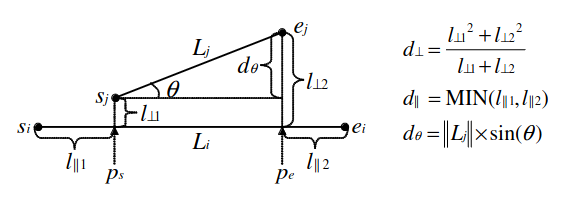
\includegraphics[width=0.44\textwidth]{Images/distances.png}
    \caption{Les 3 composantes de distance entre 2 segments}
    \label{fig:distancesA}
    Source : \href{https://hanj.cs.illinois.edu/pdf/sigmod07_jglee.pdf}{Trajectory Clustering: A Partition-and-Group Framework}
\end{figure}

\begin{enumerate}
    \item La distance perpendiculaire $d_{\perp}$ :
        \begin{equation}
            d_{\perp}(L_i, L_j) = \frac{l_{\perp 1}^2 + l_{\perp 2}^2}{l_{\perp 1} + l_{\perp 2}},
        \end{equation}
        où $l_{\perp 1}$ est la distance euclidienne entre $\overrightarrow{sj}$ et le point de projection $p_s$ de $\overrightarrow{sj}$ sur $L_i$, et $l_{\perp 2}$ est la distance euclidienne entre $\overrightarrow{ej}$ et le point de projection $p_e$ de $\overrightarrow{ej}$ sur $L_i$.



    \item La distance parallèle $d_{\parallel}$ est définie comme :
        \begin{equation}
            d_{\parallel}(L_i, L_j) = \min(l_{\parallel 1}, l_{\parallel 2}),
        \end{equation}
        où $l_{\parallel 1}$ est la distance euclidienne minimale entre $p_s$ et $\overrightarrow{si}$ ou $\overrightarrow{ei}$, et $l_{\parallel 2}$ est la distance euclidienne minimale entre $p_e$ et $\overrightarrow{si}$ ou $\overrightarrow{ei}$.


    \item La distance d'angle $d_{\theta}$ est définie comme :
        \begin{equation}
            d_{\theta}(Li, Lj ) =
            \begin{cases}
                \| Lj \| \times \sin({\theta}), & \text{si } 0^\circ \le {\theta} < 90^\circ\ \\
                \| Lj \|, & si \hspace{0.3cm} 90^\circ \le {\theta} \le 180
            \end{cases}
        \end{equation}

        où $\theta$ est l'angle d'intersection le plus petit entre $L_i$ et $L_j$ et $\| L_j \|$ est la longueur de $L_j$.

        %‖ Lj ‖


\end{enumerate}

\vspace{0.5cm}
Nous définissons finalement la distance entre deux segments de droite comme suit : 

\[
\mathrm{dist}(L_i,L_j) = w_\perp \cdot d_\perp(L_i,L_j) + w_{\parallel} \cdot d_{\parallel}(L_i,L_j) + w_\theta \cdot d_\theta(L_i,L_j)
\]

Les poids $w_\perp$, $w_{\parallel}$ et $w_\theta$ seront à déterminer en fonction des applications. Dans notre cas, nous les fixerons défaut à 1, car selon l'auteur ces valeurs fonctionnent généralement bien dans de nombreuses applications et ensembles de données.

%%%%%%%%%%%%%%%%%%%%%%%%%%%%%%%%%%%%%%%%%
\section{Compression en temps linéaire}
\label{an:compression_lin}

La méthode proposée consiste à considérer que l'ensemble des optima locaux est l'optimum global. On définira $MDLpar(p_i, p_j)$ le coût MDL ($ L(H) + L(D|H) $) d'une trajectoire entre pi et pj (i<j) en supposant que pi et pj sont les seuls points caractéristiques. Et MDLnopar(pi, pj) le coût MDL en supposant que tous les points de pi à pj sont caractéristiques, autrement dit, en préservant la trajectoire originale. Notons que dans MDLnopar(pi, pj), $L(D|H)$ est nul. Un optimum local est la partition de trajectoire pipj la plus longue qui satisfait MDLpar(pi, pk) $\le$ MDLnopar(pi, pk) pour tout k tel que $i < k \le j$. Si le premier est inférieur au second, cela signifie que choisir pk comme point caractéristique rend le coût de MDL plus petit que de ne pas le choisir.

%Approximate Trajectory Partitioning
L'algorithme fonctionne de la manière suivante :

\begin{enumerate}
    \item Nous calculons MDLpar et MDLnopar pour chaque point d'une trajectoire. 
    \item Si MDLpar est supérieur à MDLnopar, nous insérons le point précédent immédiat dans l'ensemble des points caractéristiques. Et nous répétons la même procédure à partir de ce point. 
    \item Sinon, nous augmentons la longueur d'une partition de trajectoire candidate. Et on continue
\end{enumerate}

%%%%%%%%%%%%%%%%%%%%%%%%%%%%%%%%%%%%%%%%%
%%%%%%%%%%%%%%%%%%%%%%%%%%%%%%%%%%%%%%%%%
\chapter{Propagation d'affinité}
\section{Implémentation}
\label{an:propa}
\subsubsection{Comment avons-nous implémenté cet algorithme ?}
Par soucis de lisibilité, notons :


\begin{itemize}
    \item S, la matrice de similarité.
    \item R, la matrice de responsabilité.
    \item D, la matrice de disponibilité.
\end{itemize}
% \begin{multicols}{2}
    \hspace*{13px} La structure de nos matrices est faite pour pouvoir comparer un élément d'index I à un élément d'index J, il est donc nécessaire d'utiliser une structure de liste ordonnée et fixe.\\
    Pour commencer, il nous faut remplir la matrice de similarité.
    Chacun de nos objets donnés est capable au préalable de se comparer à d'autres objets du même type.\\
    Une méthode distance nous permet donc de comparer un objet I à un objet J. \\ 
    (Voir l'algorithme implémenté \ref{sec:simcalc})\\
    % \begin{algorithmic}[1]
    %     % \State $\texttt{Méthode de calcul de la similarité$
    %     \State $E \gets \texttt{L'ensemble d'éléments}$
    %     \State $T \gets \texttt{la taille de E}$
    %     \State $S \gets \texttt{Une matrice de taille T*T}$
    %     \For{\texttt{I allant de 0 à T}}
    %         \For{\texttt{J allant de 0 à T}}
    %             \State $S(I,J) \gets \texttt{E(I).distance(E(J))}$
    %         \EndFor
    %     \EndFor
    % \end{algorithmic}
% \end{multicols}

% \begin{multicols}{2}
    Mettre à jour la matrice de responsabilité se fait une fois la similarité calculée. (voir figure \ref{fig:responsibility})\\
    De manière plus explicite, la responsabilité d'un élément i par rapport à k se calcule par sa valeur de similarité, moins la valeur maximale de la disponibilité pour les éléments i en considérant tous les autres points de données j, sauf l'élément k. De cette manière, nous pouvons quantifier l'importance d'un élément pour les autres éléments.\\
    (Voir l'algorithme implémenté \ref{sec:rescalc})\\
    % \begin{algorithmic}[1]
    %     % \State $\texttt{Méthode de calcul de la responsabilité$
    %     \State $E \gets \texttt{L'ensemble d'éléments}$
    %     \State $T \gets \texttt{la taille de E}$
    %     \State $S \gets \texttt{Une matrice de taille T*T}$
    %     \For{\texttt{I allant de 0 à T}}
    %         \For{\texttt{J allant de 0 à T}}
    %             \State $V = \texttt{S[i] + D[i]}$
    %             \State $V[i] = -\infty$ 
    %             \State $V[k] = -\infty$
    %             \State $R[i,k] = R[i,k] + (S[i,k] - max(v))$
    %         \EndFor
    %     \EndFor
    % \end{algorithmic}
    
    \hspace*{13px} Un paramètre que nous avons nommé "damping" est un paramètre d'amortissement compris entre 0 et 1 qui contrôle la quantité de propagation d'affinité entre les éléments. Nous l'appliquons à la formule de cette manière :\\ 
    \begin{equation}
        \begin{aligned}
            R\left ( i,k \right ) = R\left ( i,k \right ) * damping + S\left ( i,k \right ) - (1 - damping) * max\left \{ D\left ( i,k' \right ) + S\left ( i,k' \right ) \right \}
        \end{aligned}
    \end{equation}\\
    Plus ce paramètre tend vers 0, plus les éléments similaires ne seront regroupés qu'avec leurs voisins directs. Au contraire, plus le damping est proche de 1, plus les points de données similaires seront regroupés ensemble, indépendamment de leur position dans l'ensemble des éléments.\\
    
    Mettre à jour la matrice de disponibilité se fait une fois la responsabilité mise à jour. \\ 
    (Voir l'algorithme implémenté \ref{sec:avacalc})\\
    % \begin{algorithmic}[1]
    %     \State $E \gets \texttt{L'ensemble d'éléments}$
    %     \State $T \gets \texttt{la taille de E}$
    %     \State $R \gets \texttt{Une matrice de taille T*T}$
    %     \For{\texttt{I allant de 0 à T}}
    %         \For{\texttt{J allant de 0 à T}}
    %             \State $V \gets \texttt{prendre colone k dans R}$
    %             \If{$i\neq k$} 
    %                 \State $V[i] = -\infty$ 
    %                 \State $V[k] = -\infty$
    %                 \State $V[V < 0] = 0$
    %                 \State $D[i,k] = D[i,k] + min(0, R[k,k] + somme(V))$
    %             \Else
    %                 \State $V[k] = -\infty$
    %                 \State $V[V < 0] = 0$
    %                 \State $D[k,k] = D[k,k] + somme(V)$
    %             \EndIf
    %         \EndFor
    %     \EndFor
    % \end{algorithmic}
    R(k,k) est l'élément de la matrice de responsabilité R correspondant à la similarité entre le point k et lui-même. La somme est prise sur tous les points de données i' autres que i et j, et mesure l'influence des autres points de données sur la disponibilité du point i pour être affecté au 
    cluster contenant le point j. La fonction max est utilisée ici pour ne prendre en compte que les valeurs positives de la matrice de responsabilité, ne considérant donc que les éléments i' qui ont une similarité positive avec le point k. Enfin, la fonction min est là pour contraindre le résultat final à être négatif ou nul. Cela permet de quantifier l'importance des autres éléments pour un élément donné.\\
    \hspace*{13px} Une fois le processus de mise à jour de la responsabilité et la disponibilité répété un certain nombre de fois, nous finissons par faire l'addition matricielle de la matrice de responsabilité avec celle de disponibilité pour pouvoir en extraire les clusters et leur représentant, nous appelons cette matrice la matrice de critère. La valeur de critère la plus élevée de chaque colonne est désignée comme exemplaire et les colonnes qui partagent le même exemplaire se trouvent dans le même cluster.\\
    \hspace*{13px} Le processus de mise à jour de la responsabilité et la disponibilité sont exécutés un nombre arbitrairement de fois dans notre implémentation. Cependant, cet algorithme converge relativement rapidement, calculer la matrice de critère à chaque itération permettrait de détecter une convergence et ainsi éviter de réaliser des itérations inutiles. \\

\section{Méthode de calcul de la similarité}
\label{sec:simcalc}
\begin{algorithmic}[1]
    % \State $\texttt{Méthode de calcul de la similarité$
    \State $E \gets \texttt{L'ensemble d'éléments}$
    \State $T \gets \texttt{la taille de E}$
    \State $S \gets \texttt{Une matrice de taille T*T}$
    \For{\texttt{I allant de 0 à T}}
        \For{\texttt{J allant de 0 à T}}
            \State $S(I,J) \gets \texttt{E(I).distance(E(J))}$
        \EndFor
    \EndFor
\end{algorithmic}

\section{Méthode de calcul de la responsabilité}
\label{sec:rescalc}
\begin{algorithmic}[1]
    % \State $\texttt{Méthode de calcul de la responsabilité$
    \State $E \gets \texttt{L'ensemble d'éléments}$
    \State $T \gets \texttt{la taille de E}$
    \State $S \gets \texttt{Une matrice de taille T*T}$
    \For{\texttt{I allant de 0 à T}}
        \For{\texttt{J allant de 0 à T}}
            \State $V = \texttt{S[i] + D[i]}$
            \State $V[i] = -\infty$ 
            \State $V[k] = -\infty$
            \State $R[i,k] = R[i,k] + (S[i,k] - max(v))$
        \EndFor
    \EndFor
\end{algorithmic}

\newpage
\section{Méthode de calcul de la disponibilité}
\label{sec:avacalc}
\begin{algorithmic}[1]
    \State $E \gets \texttt{L'ensemble d'éléments}$
    \State $T \gets \texttt{la taille de E}$
    \State $R \gets \texttt{Une matrice de taille T*T}$
    \For{\texttt{I allant de 0 à T}}
        \For{\texttt{J allant de 0 à T}}
            \State $V \gets \texttt{prendre colone k dans R}$
            \If{$i\neq k$} 
                \State $V[i] = -\infty$ 
                \State $V[k] = -\infty$
                \State $V[V < 0] = 0$
                \State $D[i,k] = D[i,k] + min(0, R[k,k] + somme(V))$
            \Else
                \State $V[k] = -\infty$
                \State $V[V < 0] = 0$
                \State $D[k,k] = D[k,k] + somme(V)$
            \EndIf
        \EndFor
    \EndFor
\end{algorithmic}





\end{appendix}



\bibliographystyle{abbrv}
\bibliography{ref}
\end{document}


